% ---------------------------------------------------------------------------
%  Uma representação espectral da aritmética
%  primos, compostos e crivos em frequência
%
%  T. Bandeira, 2026
%
%  Compilar com:  pdflatex --enable-installer artigo.tex   (duas vezes)
% ---------------------------------------------------------------------------
\documentclass[11pt,a4paper]{article}

\usepackage[T1]{fontenc}
\usepackage[utf8]{inputenc}
\usepackage[brazilian]{babel}

\usepackage{amsmath,amssymb,amsthm}
\usepackage{mathtools}
\usepackage{geometry}
\geometry{margin=3.0cm}

\usepackage{graphicx}
\usepackage{booktabs}
\usepackage{array}
\usepackage{enumitem}
\usepackage[protrusion=true,expansion=false]{microtype}
\usepackage{caption}
\captionsetup{font=small,labelfont=bf,width=0.92\textwidth}

\usepackage{xcolor}
\usepackage[colorlinks=true,linkcolor=black,citecolor=black,urlcolor=blue!55!black]{hyperref}
\usepackage{url}

\usepackage{csquotes}

% --------------------------------------------------------------- ambientes
\theoremstyle{plain}
\newtheorem{teorema}{Teorema}[section]
\newtheorem{lema}[teorema]{Lema}
\newtheorem{proposicao}[teorema]{Proposição}
\newtheorem{corolario}[teorema]{Corolário}

\theoremstyle{definition}
\newtheorem{definicao}[teorema]{Definição}
\newtheorem{exemplo}[teorema]{Exemplo}
\newtheorem{problema}[teorema]{Problema}

\theoremstyle{remark}
\newtheorem{observacao}[teorema]{Observação}

\renewcommand{\proofname}{Demonstração}

% --------------------------------------------------------------- macros
\newcommand{\N}{\mathbb{N}}
\newcommand{\R}{\mathbb{R}}
\newcommand{\Z}{\mathbb{Z}}
\newcommand{\Q}{\mathbb{Q}}
\newcommand{\A}{\mathcal{A}}
\newcommand{\Seed}{\mathcal{S}}
\newcommand{\Lat}{\Lambda}
\newcommand{\PiBloco}{\Pi_k}
\DeclareMathOperator{\dist}{dist}
\DeclareMathOperator{\amp}{amp}
\DeclareMathOperator{\iso}{iso}
\DeclareMathOperator{\nuc}{nuc}
\DeclareMathOperator{\Supp}{supp}
\newcommand{\freq}[1]{f_{#1}}
\newcommand{\nfreq}[1]{\nu_{#1}}
\newcommand{\rB}{\rho}

\setlength{\parskip}{0pt}
\setlength{\abovedisplayskip}{6pt}
\setlength{\belowdisplayskip}{6pt}

% --------------------------------------------------------------- título
\title{\bfseries Uma representação espectral da aritmética\\[0.35em]
\large primos, compostos e crivos em frequência}

\author{T. Bandeira\thanks{%
Material suplementar, incluindo código, figuras em alta resolução e a
formalização em Lean~4, disponível em
\url{https://github.com/tiagobandeira/analise-espectral-primos}.}}

\date{2026}

\begin{document}

\maketitle

\begin{abstract}
\noindent
A fatoração de um inteiro é uma relação aditiva entre logaritmos. Este artigo
desenvolve essa observação como um dicionário sistemático entre a aritmética
multiplicativa de $\N$ e a geometria aditiva da reta real: cada inteiro $m\ge2$
recebe a frequência $\nfreq{m}=\log m$, a multiplicação vira soma, e a
irredutibilidade de $m$ em relação a um conjunto de primos vira a distância de
$\nfreq{m}$ a um reticulado. Mostramos que a partição em blocos binários
$A_k=[2^k,2^{k+1})$ torna esse dicionário computável: um composto de $A_k$ tem
necessariamente um fator primo abaixo de $2^k$, de modo que o bloco anterior é a
base canônica para classificar o seguinte. Determinamos então a geometria exata do
reticulado: para todo primo $q$ de $A_k$, a distância relativa de $\nfreq{q}$ ao
reticulado gerado pelos primos menores vale \emph{exatamente}
$\log(1+1/q)/\log q$, e o mínimo sobre o bloco é atingido no maior primo, com valor
assintótico $1/(q\log q)$. A demonstração é elementar e repousa num único fato: os
dois vizinhos inteiros de um primo ímpar são compostos, logo ambos pertencem ao
reticulado. Sobre essa base construímos três retratos espectrais: o desenho do
crivo num bloco (onde os primos aparecem como picos isolados e os compostos
desaparecem por subtração), a lei de resolução que governa o custo desse desenho
($t_{\max}=\Theta(2^n/n)$, e no nível local $\Theta(q)$), e o fenômeno de
\emph{contagem coerente}, em que $k$ candidatos com o mesmo núcleo produzem
amplitude exatamente $k$ vezes a de um só — um dispositivo de contagem inteira
realizado por superposição de Fourier. Fechamos com a assinatura espectral de um
par de primos e com as questões que a representação sugere.
\end{abstract}

\vspace{0.4em}
\noindent\textbf{Palavras-chave:} logaritmos, reticulados, números suaves, crivo,
transformada de Fourier, análise espectral.

\vspace{0.2em}
\noindent\textbf{MSC 2020:} 11A41, 11N35, 42A16.

\tableofcontents

\bigskip

% ===========================================================================
\section{Introdução}
% ===========================================================================

A multiplicação de inteiros é uma operação com pouca estrutura visível. A adição
na reta real tem ordem, distância e simetria; o produto em $\N$ tem apenas a
fatoração. O logaritmo é a ponte entre as duas: ele transforma produto em soma,
e é a única (a menos de escala) com essa propriedade. Este artigo percorre essa
ponte até o fim, e o que se encontra do outro lado é uma imagem — literalmente,
uma imagem em frequência — da aritmética elementar.

A pergunta de partida é simples de enunciar. Todo inteiro $m \ge 2$ tem uma
frequência natural,
\[
  \nfreq{m} \;=\; \log m ,
\]
e a fatoração única diz que $m$ é composto exatamente quando $\nfreq{m}$ pode ser
escrito como soma de frequências de inteiros menores. Ou seja: \emph{a
primalidade é a irredutibilidade de um ponto num semigrupo aditivo}. Isso, por si
só, é apenas uma reformulação. A reformulação torna-se interessante quando se
pergunta pela \emph{distância} — quão longe $\nfreq{m}$ está do semigrupo gerado
por um conjunto de primos — porque aí a aritmética ganha uma geometria, e a
geometria pode ser desenhada.

O artigo constrói três coisas.

\paragraph{O dicionário.} Na Seção~\ref{sec:dicionario} formalizamos a tradução
entre a estrutura multiplicativa de $\N$ e a estrutura aditiva da reta. O ponto
central é que ela é um isomorfismo de semigrupos sobre os números gerados por um
conjunto de primos, de modo que perguntas multiplicativas (``$m$ é divisível por
$p$?'', ``$m$ é primo?'') se tornam perguntas aditivas (``$\nfreq{m}$ está no
reticulado?'', ``$\nfreq{m}$ é gerador?'').

\paragraph{O crivo como partição.} Na Seção~\ref{sec:blocos} mostramos que a
partição de $\N$ em blocos binários
\[
  A_k \;=\; [\,2^k,\; 2^{k+1}) , \qquad k \ge 0 ,
\]
é a partição adaptada ao dicionário. O fato decisivo é elementar: \emph{todo
composto de $A_k$ tem um fator primo menor que $2^k$} (Lema~\ref{lema:bloco}). A
consequência é que cada bloco pode ser classificado usando apenas o bloco
anterior como base — e que essa base, a \emph{semente} $\Seed_k$, é exatamente a
que o dicionário exige. O crivo de Eratóstenes aparece então como um caso
particular de uma recorrência sobre blocos, sem nada de espectral.

\paragraph{A geometria exata.} A Seção~\ref{sec:geometria} é o núcleo matemático.
Definimos a distância relativa $\rB_{\Seed}(m)$ de $\nfreq{m}$ ao reticulado
gerado pelos logaritmos de $\Seed$, e determinamos seu valor \emph{exato} para os
primos de um bloco:
\begin{equation}\label{eq:rhoexato}
  \rB(q) \;=\; \frac{\log\bigl(1+1/q\bigr)}{\log q}
  \qquad \text{para todo primo } q \in A_k,\ k\ge 2 .
\end{equation}
Não é uma cota: é igualdade. E a razão é uma única observação, quase banal — os
dois vizinhos inteiros de um primo ímpar são compostos, logo ambos pertencem ao
reticulado, de modo que o ponto do reticulado mais próximo de $\nfreq{q}$ é sempre
$\log(q+1)$. O reticulado gerado pelos primos de um bloco é, na escala $1/q$,
indistinguível do conjunto de \emph{todos} os logaritmos de inteiros. Desse valor
exato saem a cota inferior uniforme
$\rB(q) \ge \bigl(2^{k+1}(k+1)\log 2\bigr)^{-1}$ para $q \in A_k$, o mínimo
$\rB_{\min}(k) = \log(1+1/q_k)/\log q_k$ (atingido no maior primo $q_k$ do bloco)
e o assintótico $\rB_{\min}(k) \sim 1/(q_k \log q_k)$.

Com isso o dicionário fica completo, e o retrato que ele permite desenhar é o das
Seções~\ref{sec:desenho} a \ref{sec:assinatura}. Três retratos, na verdade.

\paragraph{Primeiro retrato: o desenho do crivo.} Seção~\ref{sec:desenho}. Para
cada inteiro $m$ considere a função
\[
  S_m(t) \;=\; -\tfrac12 \log\!\Bigl(1 - 2\,m^{-1/2}\cos\bigl(t\nfreq{m}\bigr)
  + m^{-1}\Bigr) ,
\]
que é o logaritmo do módulo do fator $\bigl(1-m^{-s}\bigr)^{-1}$ avaliado em
$s=\tfrac12+it$. Ela oscila com frequência $\nfreq{m}/(2\pi)$ e amplitude
$\approx m^{-1/2}$. Somando sobre um bloco e subtraindo a parte devida aos
compostos, o resíduo é a soma dos $S_q$ sobre os primos do bloco — e a
transformada de Fourier desse resíduo tem exatamente um pico por primo, em
posição $\nfreq{q}/(2\pi)$ (Figura~\ref{fig:desenho}). A subtração é uma operação
aritmética simples e a imagem é fiel; o que a figura mostra é o bloco sem os
compostos, e nada mais.

\paragraph{Segundo retrato: a lei de resolução.} Seção~\ref{sec:resolucao}. Um
desenho tem custo. Para separar dois primos consecutivos $q_1<q_2$ na imagem é
necessário observar o sinal até $t_{\max} > 2\pi/\log(q_2/q_1)$ (critério de
Rayleigh). O par que impõe o maior requisito é o de menor \emph{gap relativo} —
em geral um par de gêmeos — e daí resulta que o custo do desenho de um bloco é
$\Theta(2^n/n)$, com cotas explícitas (Teorema~\ref{teo:custo}). No nível de um
primo isolado, o requisito é $\Theta(q)$: ver a irredutibilidade de $q$ custa uma
janela de tamanho proporcional a $q$. Essa é uma propriedade da representação, e
responde a uma pergunta natural de quem olha as figuras: quanto é preciso
``aumentar o zoom''.

\paragraph{Terceiro retrato: a contagem.} Seção~\ref{sec:contagem}. Há um caso em
que a representação espectral faz algo que a aritmética faz de outro modo, e o faz
com exatidão absoluta. Remova de cada inteiro de um lote o seu núcleo, isto é, a
parte formada por um conjunto fixo $P$ de primos pequenos. Se $k$ candidatos do
lote têm o mesmo núcleo $r$, então os $k$ termos resultantes são literalmente a
\emph{mesma} função de $t$, e somam $k$ vezes. A amplitude em $\nfreq r$ é
exatamente $k$ vezes a de um único termo, para qualquer janela e qualquer
resolução (Proposição~\ref{prop:ganho}). O espectro passa a ser um contador:
a altura de um pico é o número de candidatos que compartilham aquele núcleo.

\paragraph{E um quarto, menor.} Seção~\ref{sec:assinatura}. Para um par
$(p,p+2)$, a presença do tom em $\nfreq{p+2}$ é detectável com contraste que cresce
como $T/p$; pares gêmeos e pares mistos se separam, e o fundo decai como
$1/T$. É a versão local do segundo retrato.

\medskip

\paragraph{Escopo.} O objetivo do artigo é a \emph{representação}, não a
eficiência: medimos o custo de ver, e não propomos substituir a aritmética por
transformadas. A aritmética decide a primalidade de $m$ em $O(\sqrt m)$ operações;
a imagem espectral exige uma janela de tamanho $\Theta(m)$. O valor do dicionário
está em outro lugar: ele torna visíveis relações que a notação multiplicativa
esconde, e dá a cada uma delas uma lei quantitativa. As figuras deste artigo foram
feitas para serem olhadas.

\paragraph{Convenções.} $\N=\{1,2,3,\dots\}$; $p$ e $q$ sempre denotam primos;
$\log$ é o logaritmo natural; $v_p(m)$ é o expoente de $p$ em $m$. Escrevemos
$[a,b)=\{m\in\N: a\le m<b\}$ e $\#X$ para a cardinalidade de um conjunto finito
$X$. O Teorema Fundamental da Aritmética é usado livremente, e apenas ele.

% ===========================================================================
\section{O dicionário: de produto a soma}\label{sec:dicionario}
% ===========================================================================

\subsection{Frequências}

\begin{definicao}[frequência de um inteiro]\label{def:freq}
Para $m\in\N$ com $m\ge 2$, a \emph{frequência} de $m$ é
\[
  \nfreq{m} \;=\; \log m \quad\text{(em radianos por unidade de $t$),}
  \qquad
  \freq{m} \;=\; \frac{\nfreq{m}}{2\pi} \quad\text{(em ciclos).}
\]
\end{definicao}

A escolha de $\log$ como normalização não é estética: é forçada pela
multiplicação.

\begin{lema}\label{lema:homomorfismo}
A aplicação $\nfreq{}\colon \N\to[0,\infty)$ é injetora e satisfaz
\[
  \nfreq{mn} \;=\; \nfreq{m} + \nfreq{n} \qquad (m,n\in\N).
\]
Além disso, se $\prod_{i} p_i^{e_i} = \prod_{j} q_j^{f_j}$ com $p_i,q_j$ primos e
$e_i,f_j\in\N$, então os dois lados coincidem como produtos formais.
\end{lema}

\begin{proof}
A injetividade de $\log$ em $(0,\infty)$ dá a primeira parte; a segunda é
$\log(mn)=\log m+\log n$. A afirmação final é o Teorema Fundamental da
Aritmética, lido do lado logarítmico: duas decomposições com o mesmo logaritmo
têm o mesmo valor, logo a mesma fatoração.
\end{proof}

O Lema~\ref{lema:homomorfismo} diz que $\nfreq{}$ é um isomorfismo entre o
semigrupo multiplicativo $\N$ e sua imagem aditiva. Não é um isomorfismo
\emph{sobre} $\R$: a imagem é um conjunto localmente finito (Lema~\ref{lema:local})
e portanto cheio de buracos. O interesse está justamente na estrutura desses
buracos, e é o que os reticulados da próxima subseção medem.

\subsection{Reticulados e números suaves}

\begin{definicao}\label{def:reticulado}
Seja $B$ um conjunto finito de primos. O \emph{reticulado} gerado por $B$ é
\[
  \Lat(B) \;=\; \Bigl\{\textstyle\sum_{p\in B} e_p \nfreq{p}
   \;:\; e_p\in\Z_{\ge 0}\Bigr\} \;\subset\; [0,\infty).
\]
Um inteiro $m\ge1$ é \emph{$B$-suave} se todos os seus fatores primos pertencem a
$B$.
\end{definicao}

A palavra ``reticulado'' é usada no sentido de semigrupo aditivo gerado: os
geradores são os $\nfreq p$, com coeficientes inteiros não negativos. É a noção de
\emph{coin problem} aditivo, transportada para a reta por logaritmos.

\begin{lema}\label{lema:suaves}
A aplicação $\nfreq{}$ estabelece uma bijeção entre o conjunto dos inteiros
$B$-suaves e $\Lat(B)$. Em particular,
\[
  \rB_B(m)=0 \iff m \text{ é } B\text{-suave},
\]
onde $\rB_B$ é definida na Definição~\ref{def:rho}.
\end{lema}

\begin{proof}
Se $m=\prod_{p\in B}p^{e_p}$ então $\nfreq m=\sum e_p\nfreq p\in\Lat(B)$.
Reciprocamente, se $\nfreq m=\sum e_p\nfreq p$, então
$m=\prod p^{e_p}$ pelo Lema~\ref{lema:homomorfismo}, logo $m$ é $B$-suave. A
injetividade de $\nfreq{}$ dá a unicidade.
\end{proof}

\begin{lema}\label{lema:local}
Para todo $X\ge 1$, o conjunto dos inteiros $B$-suaves $\le X$ é finito. Em
particular $\Lat(B)$ não tem pontos de acumulação em $\R$: para todo $\nu\ge0$
existem somente finitos elementos de $\Lat(B)$ em $[0,\nu]$.
\end{lema}

\begin{proof}
Se $m=\prod_{p\in B}p^{e_p}\le X$ então $e_p\le \log X/\log p$ para cada $p$, de
modo que há no máximo $\prod_{p\in B}\bigl(1+\lfloor\log X/\log p\rfloor\bigr)$
tais inteiros. Como $\Lat(B)$ é a imagem desse conjunto por $\nfreq{}$ e
$\nfreq{}$ é injetora, o mesmo vale para $\Lat(B)$.
\end{proof}

O Lema~\ref{lema:local} é o que autoriza falar em \emph{distância mínima} em vez
de ínfimo: o reticulado é localmente finito, então o mínimo é sempre atingido.

\subsection{Irredutibilidade}

\begin{definicao}\label{def:irredutivel}
Seja $m\ge2$ e $B$ um conjunto de primos. Dizemos que $m$ é \emph{$B$-redutível}
se
\[
  \nfreq m \;=\; \sum_{p\in B} e_p \,\nfreq p
  \qquad\text{com } e_p\in\Z_{\ge0}\ \text{e}\ \textstyle\sum_p e_p \ge 2 ,
\]
isto é, se $m$ se escreve como produto de pelo menos dois fatores de $B$.
Caso contrário, $m$ é \emph{$B$-irredutível}.
\end{definicao}

A condição $\sum e_p\ge2$ exclui a representação trivial $m=p$ com $p\in B$.
Note que a definição é puramente aditiva na reta: ela não menciona produtos, e é
essa a razão de ela poder ser medida por distâncias.

\begin{teorema}[irredutibilidade é primalidade]\label{teo:irred}
Seja $m\ge2$ e seja $B(m)=\{p \text{ primo} : p<m\}$. Então $m$ é
$B(m)$-irredutível se, e somente se, $m$ é primo.
\end{teorema}

\begin{proof}
Se $m$ é composto, a fatoração $m=\prod p_i^{e_i}$ tem todos os $p_i<m$, e
$\sum e_i\ge2$; tomando $\nfreq{}$ obtém-se uma representação, logo $m$ é
redutível. Reciprocamente, se $\nfreq m=\sum e_p\nfreq p$ com $p<m$ e
$\sum e_p\ge2$, então $m=\prod p^{e_p}$ é um produto de pelo menos dois inteiros
maiores que $1$, logo composto.
\end{proof}

O Teorema~\ref{teo:irred} é uma reformulação, e vale dizê-lo com clareza: ele não
demonstra nada sobre primos que a fatoração única já não contenha. Sua função é
mudar de coordenadas. Na reta, ``$m$ é composto'' passa a significar ``o ponto
$\nfreq m$ é uma soma de geradores'', e ``$m$ é primo'' significa ``o ponto
$\nfreq m$ não é''. A partir daqui, perguntas de \emph{aproximação} fazem sentido.

\subsection{A versão métrica}

\begin{definicao}\label{def:rho}
Seja $m\ge2$ e $B$ um conjunto finito de primos. A \emph{distância relativa} de
$\nfreq m$ a $\Lat(B)$ é
\[
  \rB_B(m) \;=\;
  \frac{\min\bigl\{\,|\nfreq m - x| : x\in\Lat(B),\ x\neq \nfreq m\,\bigr\}}{\nfreq m}
  \;\in\;[0,1] .
\]
Quando não há ambiguidade escrevemos apenas $\rB(m)$.
\end{definicao}

O mínimo é atingido pelo Lema~\ref{lema:local}, e a normalização por $\nfreq m$
torna $\rB$ invariante por escala: ela mede o desvio \emph{relativo}, que é a
quantidade que sobrevive quando se comparam blocos de tamanhos diferentes.

\begin{corolario}\label{cor:zero}
Para $m\ge2$ e $B$ finito, tem-se $\rB_B(m)=0$ se, e somente se, $m$ é
$B$-suave. Em particular, tomando $B=B(m)$: $\rB(m)=0$ se, e somente se, $m$ é
composto.
\end{corolario}

\begin{proof}
Imediato do Lema~\ref{lema:suaves} e do Teorema~\ref{teo:irred}.
\end{proof}

A função $\rB$ é, portanto, um indicador \emph{exato} de suavidade: não é um
preditor, é um teste. A questão que ocupa as próximas seções é quanto vale
$\rB$ nos casos em que ele não é zero — isto é, quão longe do reticulado ficam os
inteiros que não são gerados por ele. A resposta, para os primos de um bloco
binário, é surpreendentemente limpa (Seção~\ref{sec:geometria}).

\begin{observacao}[o reticulado é finito, não denso]\label{obs:denso}
Seria tentador pensar que $\Lat(B)$ é denso em $[0,\infty)$, já que os $\nfreq p$
são linearmente independentes sobre $\Q$ e o semigrupo que eles geram ``deveria''
preencher a reta. Não é o caso: pelo Lema~\ref{lema:local} o reticulado é
localmente finito, e um conjunto localmente finito não tem pontos de acumulação.
O que acontece é mais interessante: os \emph{gaps} entre elementos consecutivos de
$\Lat(B)$ crescem, mas crescem devagar, e é essa taxa que controla $\rB$ nos
primos.
\end{observacao}

% ===========================================================================
\section{O crivo como partição binária}\label{sec:blocos}
% ===========================================================================

\subsection{Por que partir em blocos}

Para usar o dicionário é preciso escolher um reticulado — isto é, um conjunto
finito de primos. Qual? A resposta clássica vem da fatoração: se $m$ é composto,
o menor fator primo de $m$ não excede $\sqrt m$. Logo, para classificar $m$,
basta conhecer os primos até $\sqrt m$. O problema é que $\sqrt m$ depende de
$m$, e um reticulado que muda a cada inteiro não tem geometria.

Os blocos binários resolvem isso tornando o limite uniforme.

\begin{definicao}\label{def:bloco}
Para $k\ge1$, o \emph{bloco binário} de índice $k$ é
\[
  A_k \;=\; [\,2^k,\;2^{k+1}) \;=\; \{2^k, 2^k+1,\dots, 2^{k+1}-1\},
\]
que tem exatamente $2^k$ elementos. Denotamos por $\Pi_k$ o conjunto dos primos
de $A_k$ e por $\Seed_k$ a \emph{semente} de nível $k$,
\[
  \Seed_k \;=\; \{p \text{ primo} : p < 2^k\} .
\]
\end{definicao}

A semente é a união dos primos dos blocos anteriores:
$\Seed_k=\Pi_1\cup\Pi_2\cup\cdots\cup\Pi_{k-1}$ para $k\ge2$, com
$\Pi_1=\{2,3\}$. É essa identidade que faz da partição binária a partição
adaptada ao crivo.

\subsection{O lema do bloco}

\begin{lema}[fator pequeno]\label{lema:bloco}
Seja $k\ge1$ e $m\in A_k$ composto. Então $m$ tem um fator primo $q<2^k$.
\end{lema}

\begin{proof}
Seja $q$ o menor fator primo de $m$ e escreva $m=qs$ com $s\ge q$ (o cofator é no
mínimo $q$ porque todos os seus fatores primos são $\ge q$). Então
\[
  q^2 \;\le\; qs \;=\; m \;<\; 2^{k+1},
\]
donde $q<2^{(k+1)/2}$. Como $k\ge1$ implica $(k+1)/2\le k$, segue $q<2^k$.
\end{proof}

O Lema~\ref{lema:bloco} é o único ingrediente estrutural de toda a teoria que
segue. Ele diz que os divisores que decidem a primalidade de um elemento do bloco
$k$ estão \emph{estritamente abaixo} do bloco — nunca dentro dele. É isso que
permite construir a base por indução, sem circularidade.

\begin{teorema}[crivo por blocos]\label{teo:crivo}
Seja $k\ge1$ e $m\in A_k$. Então $m$ é primo se, e somente se, nenhum elemento
de $\Seed_k$ divide $m$.
\end{teorema}

\begin{proof}
Se $p\in\Seed_k$ divide o primo $m$, então $p=m$; mas $p<2^k\le m$, contradição.
Reciprocamente, se nenhum $p\in\Seed_k$ divide $m$ e $m$ fosse composto, o
Lema~\ref{lema:bloco} produziria um fator primo $q<2^k$, isto é, $q\in\Seed_k$,
dividindo $m$.
\end{proof}

\begin{corolario}[recursão]\label{cor:recursao}
Para $k\ge1$, $\Pi_k$ é exatamente o conjunto dos $m\in A_k$ que não são
divisíveis por nenhum elemento de $\Seed_k=\Pi_1\cup\cdots\cup\Pi_{k-1}$. Partindo
de $\Pi_1=\{2,3\}$, isso determina todos os primos por indução em $k$.
\end{corolario}

O Corolário~\ref{cor:recursao} é o crivo de Eratóstenes, lido de baixo para cima:
em vez de riscar múltiplos em toda a reta, classificamos um bloco com o crivo
acumulado dos blocos anteriores. A diferença é de organização, não de conteúdo.

\begin{observacao}[a semente é maior que o necessário]\label{obs:sementemaior}
O Lema~\ref{lema:bloco} na verdade dá $q<2^{(k+1)/2}$, de modo que bastaria tomar
como semente os primos abaixo de $2^{(k+1)/2}$ — muito menos do que $\Seed_k$.
Escolhemos $2^k$ porque, com essa escolha, a semente coincide exatamente com a
união dos blocos anteriores, e a recursão fica sem parâmetros. É uma escolha de
clareza, não de economia.
\end{observacao}

\subsection{O produto de um intervalo}

O dicionário da Seção~\ref{sec:dicionario} é sobre frequências individuais. Para
desenhar um bloco inteiro de uma só vez (Seção~\ref{sec:desenho}) precisamos de um
objeto que carregue, de uma vez, as frequências de todos os primos abaixo de um
corte. O produto de um intervalo faz isso.

\begin{definicao}\label{def:Q}
Para $p$ primo, seja $n=\lfloor\log_2 p\rfloor$, de modo que $p\in A_n$. Definimos
\[
  Q(p) \;=\; \prod_{x=2^{\,n-1}}^{p-1} x .
\]
\end{definicao}

\begin{lema}[o primorial divide]\label{lema:primorial}
Para todo primo $p\ge2$ vale
\[
  \prod_{\substack{q\ \mathrm{primo}\\ q<p}} q \;\;\Bigm|\;\; Q(p).
\]
\end{lema}

\begin{proof}
Seja $q<p$ primo. Se $q\ge2^{n-1}$, então $q$ é um dos fatores do produto, logo
divide $Q(p)$. Se $q<2^{n-1}$, o intervalo $[2^{n-1},p-1]$ contém
$p-2^{n-1}\ge 2^n-2^{n-1}=2^{n-1}>q$ inteiros consecutivos; qualquer bloco de $q$
inteiros consecutivos contém um múltiplo de $q$, logo algum fator do produto é
múltiplo de $q$. Como os primos $q<p$ são distintos, o produto deles divide
$Q(p)$.
\end{proof}

O Lema~\ref{lema:primorial} diz que $Q(p)$ carrega \emph{todos} os primos abaixo
de $p$ na sua fatoração: os que estão no intervalo, diretamente; os menores,
através de múltiplos. É essa dupla presença que a representação espectral da
Seção~\ref{sec:desenho} vai separar.

\subsection{O algoritmo e seu custo}

O Corolário~\ref{cor:recursao} é executável em poucas linhas:

\begin{center}
\begin{minipage}{0.95\textwidth}
\footnotesize
\begin{verbatim}
P <- []                      # semente, bloco a bloco
para m = 2, 3, ... , p-1:
    primo <- verdadeiro
    para b em P:
        se b*b > m: pare
        se m mod b = 0: primo <- falso; pare
    se primo: P <- P + [m]
devolva P                    # todos os primos < p
\end{verbatim}
\end{minipage}
\end{center}

O teste de parada $b^2>m$ é o Lema~\ref{lema:bloco} aplicado em tempo de execução:
nenhum divisor acima de $\sqrt m$ precisa ser testado. O custo é o da divisão de
tentativas, $O(p\sqrt p/\log p)$: a estrutura de blocos não muda a ordem
assintótica, apenas organiza a base. Registramos isso como um fato, porque ele
delimita o que a partição binária oferece — uma base canônica e uma indução limpa,
não um algoritmo novo.

A Tabela~\ref{tab:crivo} registra a verificação direta.

\begin{table}[htbp]
\centering
\small
\begin{tabular}{rrrr}
\toprule
$p$ & $n=\lfloor\log_2 p\rfloor$ & primos $<p$ & recuperados \\
\midrule
$37$    & 5  & 11   & 11 \\
$131$   & 7  & 31   & 31 \\
$503$   & 8  & 95   & 95 \\
$2\,003$& 10 & 303  & 303 \\
$8\,009$& 12 & 1\,007 & 1\,007 \\
$16\,381$& 13 & 1\,899 & 1\,899 \\
\bottomrule
\end{tabular}
\caption{Recuperação exata dos primos por blocos, sem qualquer teste de
primalidade externo. Em todos os casos a lista coincide com $\pi(p-1)$.}
\label{tab:crivo}
\end{table}

% ===========================================================================
\section{A geometria exata do reticulado}\label{sec:geometria}
% ===========================================================================

Nesta seção $k\ge2$, $\Seed_k$ é a semente da Definição~\ref{def:bloco} e
$\rB=\rB_{\Seed_k}$ é a distância relativa da Definição~\ref{def:rho}. O objetivo
é calcular $\rB$ exatamente nos primos de $A_k$.

\subsection{A distância ao inteiro mais próximo}

O reticulado $\Lat(\Seed_k)$ é, por construção, um subconjunto dos logaritmos de
inteiros maiores que $1$. Isso dá imediatamente uma cota inferior para qualquer
distância a ele: a distância ao inteiro mais próximo. O lema seguinte calcula essa
distância.

\begin{lema}[vizinho inteiro]\label{lema:vizinho}
Sejam $q,m$ inteiros com $q\ge2$, $m\ge2$ e $m\neq q$. Então
\[
  \bigl|\nfreq q-\nfreq m\bigr| \;\ge\; \log\!\Bigl(1+\frac1q\Bigr).
\]
Além disso, a igualdade é atingida em $m=q+1$.
\end{lema}

\begin{proof}
Se $m>q$, então $m\ge q+1$ e a monotonicidade de $\log$ dá
$\nfreq m-\nfreq q\ge\log(q+1)-\log q=\log(1+1/q)$.

Se $m<q$, então $m\le q-1$ e
\[
  \nfreq q-\nfreq m \;\ge\; \log q-\log(q-1) \;=\; \log\frac{q}{q-1}.
\]
Basta comparar os dois candidatos: $\frac{q}{q-1}\ge\frac{q+1}{q}$ porque
$q^2\ge (q-1)(q+1)=q^2-1$. Logo $\log\frac{q}{q-1}\ge\log(1+1/q)$, e a cota vale
nos dois casos.
\end{proof}

O Lema~\ref{lema:vizinho} é a peça central de tudo o que segue, e sua leitura
geométrica é simples: entre todos os logaritmos de inteiros, o mais próximo de
$\nfreq q$ é sempre $\nfreq{q+1}$, e a distância vale $\approx 1/q$. Nenhum
conjunto de geradores pode fazer melhor do que isso, porque o reticulado que eles
geram está contido nesse conjunto.

\subsection{Uma cota uniforme sobre o bloco}

\begin{teorema}\label{teo:cota}
Seja $k\ge1$ e $q\in\Pi_k$. Então
\[
  \rB(q) \;\ge\; \frac{1}{2^{k+1}\,(k+1)\,\log 2}.
\]
\end{teorema}

\begin{proof}
Pelo Lema~\ref{lema:vizinho} e pela definição de $\rB$,
\[
  \rB(q) \;\ge\; \frac{\log(1+1/q)}{\log q}.
\]
Usamos duas desigualdades elementares. Primeiro, $\log(1+x)\ge \frac{x}{1+x}$ para
$x>0$; com $x=1/q$ obtemos $\log(1+1/q)\ge \frac{1}{q+1}$. Segundo, como
$q<2^{k+1}$, temos $q+1\le 2^{k+1}$ e portanto
\[
  \frac{1}{q+1}\;\ge\;\frac{1}{2^{k+1}} .
\]
Finalmente $\log q<\log 2^{k+1}=(k+1)\log 2$. Combinando,
\[
  \rB(q)\;\ge\;\frac{1/(q+1)}{\log q}\;\ge\;
  \frac{2^{-(k+1)}}{(k+1)\log 2}
  \;=\;\frac{1}{2^{k+1}(k+1)\log 2}. \qedhere
\]
\end{proof}

\subsection{O valor exato}

A cota do Teorema~\ref{teo:cota} é atingida, e por um motivo que vale enunciar
separadamente: o vizinho de um primo ímpar está sempre no reticulado.

\begin{lema}\label{lema:qmaisum}
Seja $k\ge2$ e $q\in\Pi_k$. Então todo fator primo de $q+1$ é menor que $2^k$; em
outras palavras, $q+1$ é $\Seed_k$-suave.
\end{lema}

\begin{proof}
Como $q\ge3$ é ímpar, $q+1$ é par e maior que $2$, logo não é primo. Seja $r$ um
fator primo de $q+1$. Se $r=2$, então $r<2^k$ porque $k\ge2$. Se $r$ é ímpar,
escreva $q+1=rs$; como $q+1$ é par e $r$ é ímpar, $s$ é par, logo $s\ge2$ e
\[
  r\;\le\;\frac{q+1}{2}\;\le\;\frac{2^{k+1}}{2}\;=\;2^k .
\]
Sendo $r$ ímpar e $2^k$ par, segue $r<2^k$.
\end{proof}

\begin{teorema}[valor exato]\label{teo:exato}
Seja $k\ge2$ e $q\in\Pi_k$. Então
\[
  \rB(q) \;=\; \frac{\log\bigl(1+1/q\bigr)}{\log q} .
\]
\end{teorema}

\begin{proof}
A desigualdade $\ge$ é o Lema~\ref{lema:vizinho}, pois todo elemento de
$\Lat(\Seed_k)$ é o logaritmo de um inteiro maior que $1$, e esse inteiro não é
$q$ (o reticulado é gerado por primos menores que $q$).

Para $\le$, o Lema~\ref{lema:qmaisum} diz que $q+1=\prod_{p\in\Seed_k}p^{e_p}$,
logo $\nfreq{q+1}=\sum e_p\nfreq p\in\Lat(\Seed_k)$. Como
\[
  \bigl|\nfreq q-\nfreq{q+1}\bigr| = \log\Bigl(1+\frac1q\Bigr),
\]
o mínimo que define $\rB(q)$ não excede esse valor.
\end{proof}

O Teorema~\ref{teo:exato} é o resultado central do artigo, e a sua demonstração
tem duas linhas de conteúdo: a distância não pode ser menor que a distância ao
inteiro mais próximo, e o inteiro mais próximo está sempre disponível. O
reticulado gerado pelos primos de um bloco é, na escala $1/q$, exatamente tão fino
quanto o conjunto de todos os logaritmos de inteiros. Não há como escolher uma
base melhor.

\subsection{O mínimo sobre o bloco}

\begin{definicao}\label{def:g}
Para $q\ge2$ seja
\[
  g(q) \;=\; \frac{\log(1+1/q)}{\log q}, \qquad q_k=\max\Pi_k .
\]
\end{definicao}

\begin{corolario}\label{cor:min}
Para $k\ge2$, $\rB_{\min}(k)=\min_{q\in\Pi_k}\rB(q)$ é atingido em $q_k$ e vale
\[
  \rB_{\min}(k) \;=\; g(q_k) \;=\; \frac{\log(1+1/q_k)}{\log q_k}.
\]
\end{corolario}

\begin{proof}
Pelo Teorema~\ref{teo:exato}, $\rB(q)=g(q)$ em $\Pi_k$. A função $g$ é estritamente
decrescente em $[2,\infty)$: o numerador $\log(1+1/q)$ decresce e o denominador
$\log q$ cresce, ambos positivos. Logo o mínimo de $g$ sobre $\Pi_k$ é $g(q_k)$.
\end{proof}

\begin{corolario}\label{cor:assint}
Para $k\ge2$,
\[
  \frac{1}{2^{k+1}(k+1)\log 2} \;\le\; \rB_{\min}(k) \;\le\;
  \frac{1}{q_k\log q_k}\Bigl(1+O\bigl(q_k^{-1}\bigr)\Bigr),
\]
e portanto $\rB_{\min}(k)\asymp 1/(q_k\log q_k)$, isto é,
$\rB_{\min}(k)=\Theta\bigl(2^{-k}/k\bigr)$.
\end{corolario}

\begin{proof}
A cota inferior é o Teorema~\ref{teo:cota}. Para a superior, use
$\log(1+x)\le x$: $g(q_k)\le 1/(q_k\log q_k)$. Como
$2^k\le q_k<2^{k+1}$, tem-se $q_k\asymp 2^k$ e $\log q_k\asymp k$.
\end{proof}

A Tabela~\ref{tab:rho} compara o valor exato com a cota. A convergência é rápida:
a razão entre os dois é $1{,}03$ já em $k=4$ e $1{,}000$ em $k=16$.

\begin{table}[htbp]
\centering
\small
\begin{tabular}{rrrrr}
\toprule
$k$ & $q_k$ & $\rB_{\min}(k)$ & $\bigl(2^{k+1}(k+1)\log 2\bigr)^{-1}$ & razão \\
\midrule
4  & $31$      & $9{,}245\times10^{-3}$ & $9{,}017\times10^{-3}$ & 1,025 \\
6  & $127$     & $1{,}619\times10^{-3}$ & $1{,}610\times10^{-3}$ & 1,006 \\
8  & $509$     & $3{,}149\times10^{-4}$ & $3{,}131\times10^{-4}$ & 1,006 \\
10 & $2\,039$  & $6{,}434\times10^{-5}$ & $6{,}404\times10^{-5}$ & 1,005 \\
12 & $8\,191$  & $1{,}355\times10^{-5}$ & $1{,}355\times10^{-5}$ & 1,000 \\
14 & $32\,749$ & $2{,}937\times10^{-6}$ & $2{,}935\times10^{-6}$ & 1,001 \\
16 & $131\,071$& $6{,}475\times10^{-7}$ & $6{,}475\times10^{-7}$ & 1,000 \\
\bottomrule
\end{tabular}
\caption{O mínimo de $\rB$ sobre o bloco e a cota do Teorema~\ref{teo:cota}.}
\label{tab:rho}
\end{table}

\begin{figure}[htbp]
\centering
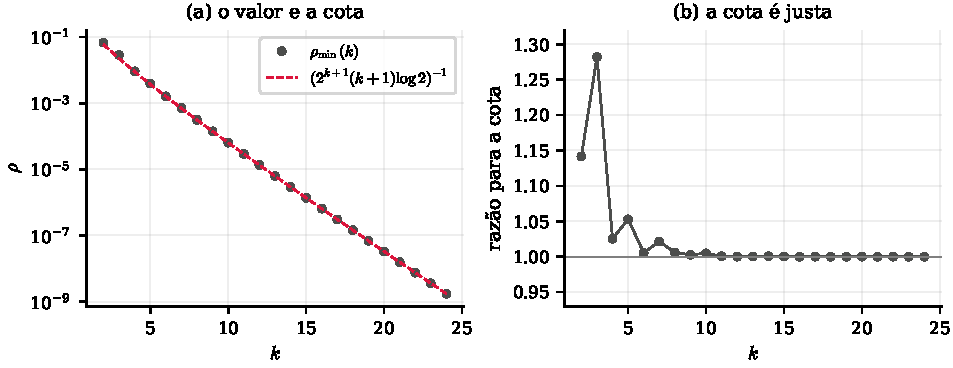
\includegraphics[width=0.95\textwidth]{figuras/f4_reticulado.pdf}
\caption{(a) $\rB_{\min}(k)$ e a cota do Teorema~\ref{teo:cota}, em escala
logarítmica. (b) A razão entre os dois; as oscilações nos blocos pequenos são os
saltos de $q_k$ quando o topo do bloco deixa de ser primo.}
\label{fig:reticulado}
\end{figure}

\subsection{O reticulado separa, e a margem é exata}

Juntando o Teorema~\ref{teo:exato} com o Corolário~\ref{cor:zero} obtém-se a
descrição completa da função $\rB$ sobre um bloco.

\begin{corolario}[os dois valores de $\rB$]\label{cor:doisvalores}
Seja $k\ge2$. Para $m\in A_k$:
\[
  \rB(m) \;=\;
  \begin{cases}
    0, & \text{se } m \text{ é composto},\\[2pt]
    g(m), & \text{se } m \text{ é primo}.
  \end{cases}
\]
Em particular, para todo $\theta$ com $0<\theta<\rB_{\min}(k)$,
\[
  \{m\in A_k : \rB(m) > \theta\} \;=\; \Pi_k .
\]
\end{corolario}

\begin{proof}
Se $m$ é composto, o Lema~\ref{lema:bloco} garante que todos os seus fatores
primos estão em $\Seed_k$, logo $m$ é $\Seed_k$-suave e
$\rB(m)=0$ pelo Corolário~\ref{cor:zero}. Se $m$ é primo, o
Teorema~\ref{teo:exato} dá $\rB(m)=g(m)>0$. A segunda afirmação segue porque $g$
é positiva e $\rB_{\min}(k)$ é o seu mínimo sobre $\Pi_k$.
\end{proof}

A leitura do Corolário~\ref{cor:doisvalores} merece cuidado, porque é fácil
transformá-la em algo que ela não diz. O que ele afirma é que a separação é
\emph{perfeita e com margem}: os compostos dão exatamente zero e os primos dão no
mínimo $\rB_{\min}(k)$. Todo limiar $\theta$ estritamente entre esses dois níveis
classifica corretamente o bloco inteiro. A margem, isto é, a distância entre os
dois níveis, vale exatamente
\[
  \rB_{\min}(k) \;=\; \frac{\log(1+1/q_k)}{\log q_k} \;\sim\; \frac{1}{q_k\log q_k},
\]
e é essa quantidade — e não outra — que mede a resolução com que a geometria
logarítmica distingue um primo de um composto. Ela decai como $1/(q\log q)$ com o
tamanho do primo, o que é o preço intrínseco da representação.

Não há, portanto, um \emph{gradiente} de primalidade: fora do conjunto dos primos,
$\rB$ é identicamente nulo sobre o bloco. Um inteiro composto de $A_k$ não está
``quase'' no reticulado — está nele, exatamente, e a distância zero é o conteúdo
aritmético do Lema~\ref{lema:bloco} traduzido para a reta.

\subsection{Por que a rota diofantina é desnecessária}

A cota do Teorema~\ref{teo:cota} poderia, em princípio, ser obtida pela teoria de
formas lineares em logaritmos, que fornece minorantes para
$\bigl|\sum e_i\nfreq{p_i}-\nfreq m\bigr|$ quando $m$ não é o produto
correspondente \cite{baker}. Essas cotas são da ordem de
$\exp\bigl(-C\,k\log^2 2\log k\bigr)$ — duplamente exponenciais em $k$ —, e para
$k=16$ ficam dezenas de ordens de grandeza abaixo do valor real.

A razão da discrepância é instrutiva. Os teoremas de formas lineares controlam o
\emph{pior caso} de uma combinação inteira arbitrária de logaritmos de primos.
Aqui o objeto não é arbitrário: queremos a distância de $\nfreq q$ ao conjunto dos
$\nfreq m$ com $m$ inteiro, e os inteiros são ordenados. A ordenação resolve o
problema: o vizinho é sempre $q+1$, e não há nada a estimar. Toda a dificuldade da
aproximação diofantina vem de permitir coeficientes negativos e geradores
arbitrários; a restrição ao reticulado dos inteiros elimina essa dificuldade.

Vale sublinhar o contraste, porque ele é o resumo matemático desta seção: o
problema \emph{geral} de aproximar logaritmos por combinações inteiras é profundo;
o problema \emph{restrito} que a aritmética formula é elementar. E é justamente a
restrição — o fato de o reticulado ser gerado pelos mesmos inteiros que se quer
classificar — que explica por que a irredutibilidade logarítmica, como problema de
aproximação, não carrega dificuldade diofantina alguma.

% ===========================================================================
\section{O desenho do crivo}\label{sec:desenho}
% ===========================================================================

Temos um dicionário (Seção~\ref{sec:dicionario}) e uma base canônica para cada
bloco (Seção~\ref{sec:blocos}). Falta o instrumento que torna o dicionário
visível. Ele vem, sem surpresa, do fator de Euler.

\subsection{O tom de um inteiro}

Seja $s=\tfrac12+it$ com $t\in\R$. Para $m\ge2$,
\[
  \bigl|1-m^{-s}\bigr|^2
  \;=\; 1-2\,m^{-1/2}\cos\bigl(t\nfreq m\bigr)+m^{-1},
\]
de modo que o logaritmo do módulo do fator de Euler correspondente é
\begin{equation}\label{eq:Sm}
  S_m(t) \;=\; -\tfrac12\log\!\Bigl(1-2\,m^{-1/2}\cos\bigl(t\nfreq m\bigr)+m^{-1}\Bigr).
\end{equation}

\begin{lema}[série de Fourier de $S_m$]\label{lema:serie}
Para todo $t\in\R$,
\begin{equation}\label{eq:serie}
  S_m(t) \;=\; \sum_{k\ge1}\frac{m^{-k/2}}{k}\,\cos\bigl(k\,t\,\nfreq m\bigr).
\end{equation}
Em particular $S_m$ é limitada e positiva, e sua componente fundamental oscila
com frequência $\freq m=\nfreq m/2\pi$ e amplitude $m^{-1/2}$.
\end{lema}

\begin{proof}
Com $a=m^{-1/2}\in(0,1)$ e $\theta=t\nfreq m$, a identidade clássica
$\log(1-2a\cos\theta+a^2)=-2\sum_{k\ge1}\frac{a^k}{k}\cos(k\theta)$ — que segue da
série de $\log(1-z)$ em $|z|<1$, tomando $z=ae^{i\theta}$ e $z=ae^{-i\theta}$ e
somando — dá \eqref{eq:serie} após multiplicar por $-\tfrac12$.
\end{proof}

A série \eqref{eq:serie} é a tradução sonora do dicionário. O inteiro $m$ emite um
tom fundamental na sua frequência e harmônicos nos múltiplos inteiros dessa
frequência, com amplitudes que decaem geometricamente. Um composto emite, por
construção, um tom fundamental que é a \emph{soma} das frequências dos seus
fatores — o que o Lema~\ref{lema:homomorfismo} garante — e cujos harmônicos também
coincidem com combinações das frequências dos fatores.

\subsection{Ortogonalidade}

\begin{lema}[ortogonalidade]\label{lema:orto}
Sejam $\alpha,\beta>0$ e $T>0$. Então
\[
  \frac1T\int_0^T\cos(\alpha t)\cos(\beta t)\,dt
  =
  \begin{cases}
    \dfrac12+O\!\left(\dfrac{1}{T\alpha}\right), & \alpha=\beta,\\[10pt]
    O\!\left(\dfrac{1}{T|\alpha-\beta|}\right), & \alpha\neq\beta .
  \end{cases}
\]
\end{lema}

\begin{proof}
A identidade de produto de cossenos reduz a integral a
$\tfrac12\int_0^T\cos((\alpha-\beta)t)\,dt+\tfrac12\int_0^T\cos((\alpha+\beta)t)\,dt$,
e $\bigl|\int_0^T\cos(\gamma t)\,dt\bigr|\le 2/|\gamma|$ para $\gamma\neq0$,
enquanto $\int_0^T1\,dt=T$.
\end{proof}

O Lema~\ref{lema:orto} é o que autoriza ler amplitudes: sobre uma janela longa, o
coeficiente de um sinal em uma frequência é determinado — a menos de $O(1/T)$ —
pela componente que oscila exatamente naquela frequência. As frequências
$\nfreq m$ de inteiros distintos nunca coincidem, porque $\nfreq{}$ é injetora.

\subsection{O resíduo de um bloco}

Seja $I$ um conjunto finito de inteiros e defina
\[
  Z_I(t) \;=\; \sum_{m\in I} S_m(t).
\]
Para $p$ primo com $n=\lfloor\log_2 p\rfloor$, tome o intervalo
$I_p=[2^{n-1},p-1]$ e separe-o em primos e compostos:
$I_p = \Pi \sqcup C$, com $\Pi=\{q\in I_p: q \text{ primo}\}$ e $C$ o resto. Então
\begin{equation}\label{eq:residuo}
  R(t) \;=\; Z_{I_p}(t)-Z_C(t) \;=\; Z_{\Pi}(t) \;=\; \sum_{q\in\Pi} S_q(t).
\end{equation}

A identidade \eqref{eq:residuo} é exata, para todo $t$, por linearidade da soma:
subtrair o sinal dos compostos remove exatamente esses termos e não toca nos
demais. Não há aproximação envolvida \emph{na construção}. O que há é uma escolha
de representação: em vez de olhar $Z_{I_p}$, olhamos o resíduo, que contém apenas
os tons dos primos do bloco.

A Figura~\ref{fig:desenho} mostra o resultado para $p=37$, isto é,
$I_p=[16,36]$. À esquerda, o espectro de $Z_{I_p}$: vinte e uma oscilações
superpostas, sem estrutura legível. À direita, o espectro de $R$: cinco picos
isolados, e eles estão exatamente nas frequências dos cinco primos do intervalo —
$17,19,23,29,31$.

\begin{figure}[htbp]
\centering
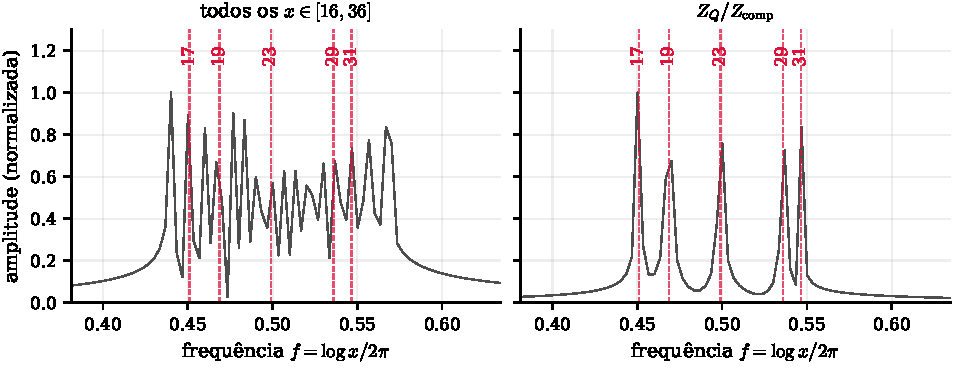
\includegraphics[width=0.98\textwidth]{figuras/f1_desenho.pdf}
\caption{O bloco $I_p=[16,36]$ de $Q(37)$, com $t_{\max}=300$ e passo
$\Delta t=0{,}02$. À esquerda, o espectro de $Z_{I_p}$, que soma os vinte e um
inteiros do intervalo. À direita, o resíduo \eqref{eq:residuo}, obtido subtraindo
o sinal dos compostos: restam os tons dos cinco primos, nas posições previstas
pelo dicionário.}
\label{fig:desenho}
\end{figure}

Vale registrar o que a figura \emph{não} faz. Ela não decide primalidade: a
subtração em \eqref{eq:residuo} usa a lista $\Pi$, isto é, usa a informação
aritmética que se quer representar. O que a figura oferece é uma
\emph{representação} dessa informação — uma em que cada primo é um objeto visual
distinguível, com posição e altura determinadas pela sua frequência e pelo seu
tamanho.

\subsection{A outra metade do reticulado}

O resíduo \eqref{eq:residuo} contém os primos do intervalo $I_p$, isto é, os
primos entre $2^{n-1}$ e $p$. Os primos menores — a semente $\Seed_{n}$ — não
estão lá como tons diretos. Eles aparecem, porém, de outra forma: como
\emph{divisores} dos compostos de $I_p$, e portanto como frequências presentes no
sinal dos compostos que acabamos de subtrair.

Há uma maneira clássica de extrair essa contribuição: comparar $Z_{I_p}$ com a
função zeta, cujo produto de Euler percorre todos os primos \cite{titchmarsh}. A
diferença
\[
  Z_{I_p}(t)-\log\bigl|\zeta(\tfrac12+it)\bigr|
\]
cancela os primos do intervalo, que aparecem nos dois lados, e deixa visíveis os
primos pequenos, que no intervalo aparecem apenas através de múltiplos. O preço é
ter de avaliar $\zeta$ na linha crítica em precisão suficiente, o que é caro; e a
alternativa aritmética da Seção~\ref{sec:blocos} obtém a semente por recursão, sem
números complexos.

Mencionamos o artifício porque ele fecha a imagem: o dicionário comporta as duas
metades do reticulado, os primos do bloco como tons diretos e a semente como
ressonância nos compostos. A Figura~\ref{fig:desenho} mostra a primeira metade; a
segunda é mais difícil de ver e não a usaremos adiante.

\subsection{Quanta resolução é necessária}

Um pico é um objeto de largura finita. A janela de observação $[0,T]$ dá à
transformada uma resolução em frequência da ordem de $1/T$ (Lema~\ref{lema:orto}),
e dois primos consecutivos $q_1<q_2$ só aparecem como picos separados se
\[
  \frac{1}{T} \;\ll\; \freq{q_2}-\freq{q_1}
  \;=\; \frac{\log(q_2/q_1)}{2\pi} .
\]
Isso é o conteúdo da próxima seção, onde a desigualdade é tornada exata e o custo
do desenho é calculado. A Figura~\ref{fig:resolucao} antecipa o efeito: o mesmo
bloco de $Q(53)$, desenhado com duas janelas diferentes, revela ou esconde os
pares mais próximos.

\begin{figure}[htbp]
\centering
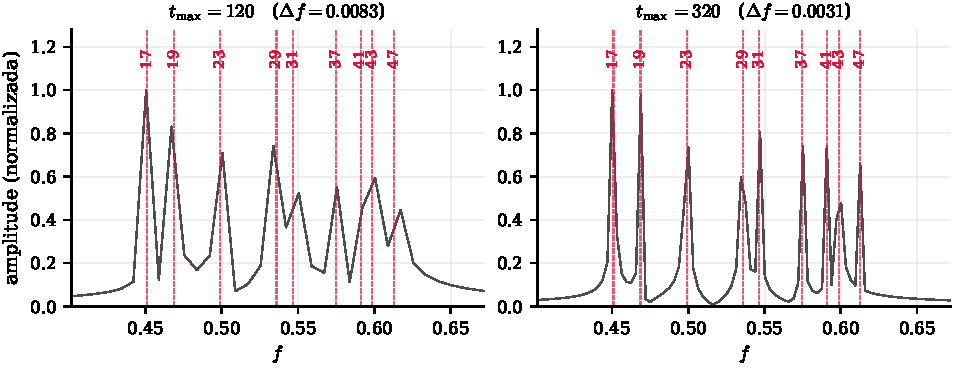
\includegraphics[width=0.98\textwidth]{figuras/f2_resolucao.pdf}
\caption{O bloco $I_p=[32,52]$ de $Q(53)$ com duas janelas. À esquerda,
$t_{\max}=120$: os pares de primos consecutivos mais próximos aparecem fundidos,
e o desenho conta menos picos do que primos. À direita, $t_{\max}=320$: todos os
primos do bloco são resolvidos. A posição dos picos é a mesma nos dois casos; o
que muda é a capacidade de separá-los.}
\label{fig:resolucao}
\end{figure}

% ===========================================================================
\section{A resolução: quanto custa ver}\label{sec:resolucao}
% ===========================================================================

Um pico é um objeto de largura finita, e a largura é determinada pela janela de
observação. Nesta seção tornamos essa afirmação quantitativa, obtemos a lei de
escala do desenho de um bloco e o custo de ver um único primo.

\subsection{O critério de Rayleigh}

Sejam dois tons de frequências $\nu_1<\nu_2$ (em radianos) e amplitudes $a_1,a_2$,
observados em $[0,T]$. O coeficiente de um tom na frequência do outro é regido
pelo núcleo de Dirichlet.

\begin{lema}\label{lema:kernel}
Com $\delta=\nu_2-\nu_1>0$ e $T>0$,
\[
  \left|\int_0^T\cos(\nu_2 t)\,e^{-i\nu_1 t}\,dt\right|
  \;=\;
  \left|\frac{\sin(\delta T/2)}{\delta/2}\right|\cdot\bigl(1+O((T\nu_1)^{-1})\bigr).
\]
Em particular o coeficiente se anula quando $\delta T/(2\pi)\in\Z\setminus\{0\}$ e
vale $\approx T/2$ quando $\delta T\ll1$.
\end{lema}

\begin{proof}
Escreva $2\cos(\nu_2t)=e^{i\nu_2t}+e^{-i\nu_2t}$ e integre $e^{i(\nu_2-\nu_1)t}$ e
$e^{-i(\nu_2+\nu_1)t}$; a primeira integral vale
$\bigl|e^{i\delta T}-1\bigr|/\delta=2|\sin(\delta T/2)|/\delta$, a segunda é
$O(1/(\nu_1+\nu_2))$.
\end{proof}

O Lema~\ref{lema:kernel} diz que a largura do lóbulo principal de um pico, medida
entre os dois zeros vizinhos, é $2\pi/T$ em radianos, isto é, $1/T$ em ciclos.
Dois tons são \emph{resolvidos} quando o pico de um não cai dentro do lóbulo
principal do outro, o que dá o critério clássico.

\begin{lema}[Rayleigh]\label{lema:rayleigh}
Para que dois tons de frequências $\freq{q_1}<\freq{q_2}$ apareçam como picos
distintos numa janela de comprimento $T$, é necessário
\[
  T \;>\; \frac{2\pi}{\log(q_2/q_1)} \;=\; \frac{1}{\freq{q_2}-\freq{q_1}} .
\]
\end{lema}

\begin{proof}
O primeiro zero do núcleo do Lema~\ref{lema:kernel} ocorre em
$\delta T=2\pi$, isto é, $T=1/(\freq{q_2}-\freq{q_1})$.
\end{proof}

\subsection{O par gargalo e a lei de escala}

Pelo Lema~\ref{lema:rayleigh}, o comprimento de janela exigido por um par é
$2\pi/\log(q_2/q_1)$, tanto maior quanto menor for o \emph{gap relativo}
$\log(q_2/q_1)=\log(1+g/q_1)$ do par. Para primos consecutivos, $g\ge2$, e a
igualdade $g=2$ caracteriza os pares de gêmeos.

\begin{definicao}\label{def:gargalo}
Para um conjunto finito $\Seed$ de primos com $\#\Seed\ge2$, o \emph{par gargalo} é
o par de primos consecutivos $q_1<q_2$ de $\Seed$ que maximiza
$2\pi/\log(q_2/q_1)$, e
\[
  \tau(\Seed) \;=\; \frac{2\pi}{\max\log(q_2/q_1)}
\]
é a \emph{janela exigida} por $\Seed$.
\end{definicao}

\begin{teorema}[lei de escala]\label{teo:custo}
Seja $Q_k=\max \Seed_k$ (o maior primo abaixo de $2^k$) e $m_k=\#\Seed_k$. Então
\[
  \frac{2\pi}{\log\bigl(1+2/(Q_k-2)\bigr)}
  \;\le\; \tau(\Seed_k) \;\le\; 2\pi\,(m_k-1),
\]
e, como $m_k\asymp 2^k/k$ e $Q_k\asymp 2^k$, vale
$\tau(\Seed_k)=\Theta(2^k/k)$ com constantes explícitas.
\end{teorema}

\begin{proof}
\emph{Cota superior.} Seja $q_1<q_2$ um par qualquer de $\Seed_k$, com gap
$g=q_2-q_1\ge2$. Como $q_1\le Q_k-2$, temos $g/q_1\ge 2/(Q_k-2)$, donde
$\log(q_2/q_1)=\log(1+g/q_1)\ge\log(1+2/(Q_k-2))$ e portanto
$2\pi/\log(q_2/q_1)\le 2\pi/\log(1+2/(Q_k-2))$.

\emph{Cota inferior.} Os $m_k$ elementos de $\Seed_k$ estão todos em
$[2,Q_k-1]$, um intervalo de comprimento $Q_k-2$; logo algum par de consecutivos
tem gap $g\le (Q_k-2)/(m_k-1)$. Para esse par,
$\log(q_2/q_1)=\log(1+g/q_1)\le g/q_1\le 1/(m_k-1)$, e assim
$2\pi/\log(q_2/q_1)\ge 2\pi(m_k-1)$.

\emph{Assintótica.} Pelo teorema dos números primos $m_k\sim 2^k/(k\log2)$, e
$2^{k-1}<Q_k<2^k$; substituindo nas duas cotas obtém-se o mesmo expoente.
\end{proof}

Em palavras: a janela necessária para desenhar um bloco cresce como $2^k/k$, isto
é, essencialmente como o próprio bloco dividido por um fator logarítmico. A
Figura~\ref{fig:lei} mostra as duas pontas do Teorema~\ref{teo:custo} para
$k=4,\dots,22$: a curva medida cresce exponencialmente e, o que é mais preciso,
coincide com $\pi q_{\text{gêmeo}}$, onde $q_{\text{gêmeo}}$ é o maior elemento de
um par de gêmeos da semente.

\begin{figure}[htbp]
\centering
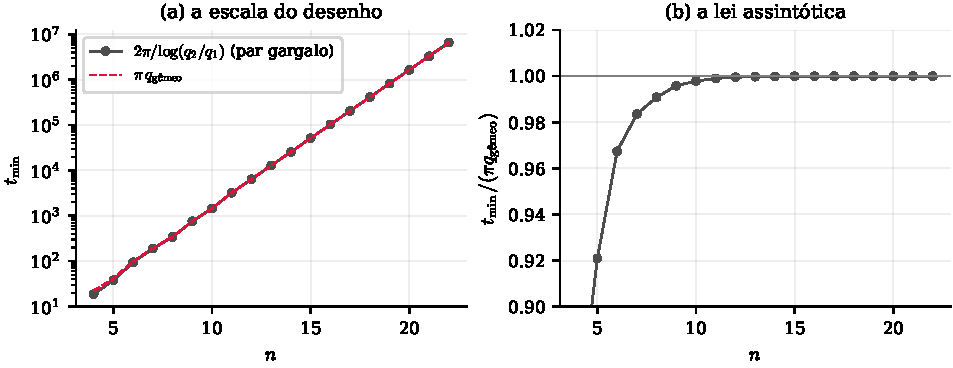
\includegraphics[width=0.95\textwidth]{figuras/f3_lei.pdf}
\caption{(a) A janela exigida pelo par gargalo de $\Seed_k$, em escala
logarítmica; a curva é indistinguível de $\pi q_{\text{gêmeo}}$. (b) A razão entre
os dois tende a $1$: o erro relativo já é $10^{-3}$ em $n=9$.}
\label{fig:lei}
\end{figure}

\begin{table}[htbp]
\centering
\footnotesize
\begin{tabular}{rrrrr}
\toprule
$n$ & par gargalo & janela exigida & $\pi\,q_{\text{gêmeo}}$ & razão \\
\midrule
6  & $(29,\,31)$        & $94{,}2$      & $97{,}4$      & 0,967 \\
8  & $(107,\,109)$      & $339{,}3$     & $342{,}4$     & 0,991 \\
10 & $(461,\,463)$      & $1\,451{,}4$  & $1\,454{,}6$  & 0,998 \\
12 & $(2\,027,\,2\,029)$& $6\,371{,}1$  & $6\,374{,}3$  & 0,9995 \\
14 & $(8\,087,\,8\,089)$& $25\,409{,}2$ & $25\,412{,}3$ & 0,9999 \\
\bottomrule
\end{tabular}
\caption{O par gargalo é sempre um par de gêmeos nas escalas verificadas, e a
janela exigida coincide com $\pi q_{\text{gêmeo}}$ no limite.}
\label{tab:lei}
\end{table}

\subsection{O custo de ver um primo}

O Teorema~\ref{teo:custo} é sobre um bloco inteiro. Há uma versão local, que é a
que responde à pergunta ``quanto custa verificar que $q$ é primo olhando o
espectro?''.

\begin{corolario}[custo local]\label{cor:local}
Seja $q\ge5$ primo e considere o sinal $R$ definido em \eqref{eq:Rprimo}, com
$N\ge q$. Para decidir, com margem constante, se o tom de frequência $\nfreq q$
está presente, é necessário uma janela $T=\Omega(q)$; e $T$ proporcional a $q$
com constante adequada é suficiente.
\end{corolario}

\begin{proof}
A prova é a Proposição~\ref{prop:gemeo} da Seção~\ref{sec:assinatura}, que
quantifica o resíduo: na ausência do tom — isto é, se $q$ não está na soma — a
amplitude relativa em $\nfreq q$ é $O(q/T)$, enquanto a presença do tom dá
$1+O(\sqrt q/T)$. Separar os dois com margem fixa exige $T\gg q$, e $T$
proporcional a $q$ com constante adequada basta.
\end{proof}

O contraste com a aritmética é o ponto. A divisão de tentativas decide a
primalidade de $q$ em $O(\sqrt q)$ operações, sem sinal e sem janela. Ver $q$ no
espectro custa uma janela de comprimento proporcional a $q$. O fator entre as duas
escalas é $\sqrt q$: é o preço, em resolução, de representar a irredutibilidade
como uma propriedade de frequência em vez de uma propriedade de divisibilidade.

Isso não é um defeito da construção — é uma medida. O dicionário da
Seção~\ref{sec:dicionario} é fiel, e a fidelidade tem este custo: para separar
$\nfreq q$ do tom do primo vizinho, cuja distância relativa é $\approx 2/q$, a
janela precisa ser da ordem de $q$.

\subsection{A janela de leitura}

Na prática, para localizar um pico mede-se o máximo da amplitude em uma faixa de
$\pm W$ células em torno da frequência procurada. Essa escolha introduz um segundo
parâmetro, que não tem nada a ver com $T$ e que pode arruinar a leitura.

\begin{proposicao}[janela de leitura]\label{prop:janela}
Seja $q\ge5$ primo e $\delta=\log\bigl(q/(q-2)\bigr)$ a distância entre as
frequências de $q$ e de $q-2$. Para que a faixa de $\pm W$ células em torno de
$\freq q$ não contenha o lóbulo principal do pico de $q-2$, é necessário
\[
  2W+1 \;<\; \frac{T\,\delta}{2\pi} \;\approx\; \frac{T}{\pi q} .
\]
\end{proposicao}

\begin{proof}
É o Lema~\ref{lema:rayleigh} aplicado ao par $(q-2,q)$, com a largura $2W+1$ da
faixa no lugar de uma célula, e $\delta=\log(1+2/(q-2))\ge 2/q$.
\end{proof}

A Proposição~\ref{prop:janela} explica por que medidas com a mesma janela $T$
podem discordar: se a faixa de leitura for larga em relação ao gap, o máximo lido
em $\freq q$ é o pico do vizinho. Para $q\approx300$ e $T=6500$, o lado direito
vale $6{,}9$ células; uma leitura com $W=2$ é segura, uma com $W=10$ não é. A
Tabela~\ref{tab:janela} registra o efeito.

\begin{table}[htbp]
\centering
\small
\begin{tabular}{rrrrr}
\toprule
$T$ & $W=0$ & $W=2$ & $W=10$ & $T/(\pi q_{\max})$ \\
\midrule
$1\,500$ & $100\%$ & $77\%$ & $42\%$ & $1{,}6$ \\
$6\,500$ & $100\%$ & $100\%$ & $77\%$ & $6{,}9$ \\
\bottomrule
\end{tabular}
\caption{Acurácia da separação entre pares gêmeos e mistos
(Seção~\ref{sec:assinatura}) em função da meia-largura $W$ da faixa de leitura,
para $N=300$. A separação sobrevive enquanto $2W+1<T/(\pi q_{\max})$.}
\label{tab:janela}
\end{table}

% ===========================================================================
\section{A contagem coerente}\label{sec:contagem}
% ===========================================================================

As seções anteriores desenham o crivo. Esta descreve um caso em que a
representação espectral deixa de ser um desenho e passa a ser um instrumento de
\emph{medição}, com uma propriedade que a aritmética não tem de graça: a altura de
um pico é uma contagem exata.

\subsection{Núcleos e órbitas}

Fixe um conjunto finito $P$ de primos, que chamaremos de \emph{base de remoção}.
Para $m\in\N$, o \emph{núcleo} de $m$ em relação a $P$ é a parte que sobra quando
se removem todos os fatores de $P$:
\[
  \nuc_P(m) \;=\; \frac{m}{\prod_{p\in P}p^{\,v_p(m)}} .
\]
A \emph{órbita} de um inteiro $P$-livre $r$ é
\[
  \mathcal{O}_r \;=\; \bigl\{\,m\in\N : \nuc_P(m)=r\,\bigr\}
  \;=\; \Bigl\{\,r\prod_{p\in P}p^{a_p} \in \N \,\Bigr\}_{a_p\ge0} .
\]
A órbita é a classe de equivalência de $m$ pela relação ``tem a mesma parte livre
de $P$''. Todos os seus elementos têm, por construção, o mesmo núcleo.

\begin{observacao}\label{obs:orbita}
A órbita $\mathcal O_r$ é o conjunto dos elementos de $\Lat(P)$ transladados de
$\nfreq r$. Em particular, se $r$ é um primo que não está em $P$, então $\nfreq r$
não pertence a $\Lat(P)$: o núcleo de $r$ é ele mesmo, e a órbita de $r$ é o
próprio $r$.
\end{observacao}

\subsection{A identidade de contagem}

Seja $\varphi\colon\N\to(0,\infty)$ uma função de peso, e considere o sinal
formado pela soma dos tons de todos os elementos de um lote $\mathcal L$, cada um
emitido na frequência do seu \emph{núcleo}:
\begin{equation}\label{eq:colapsado}
  R_{\mathcal L}(t) \;=\;
  \sum_{\substack{m\in\mathcal L\\ \nuc_P(m)>1}}
  \varphi\bigl(\nuc_P(m)\bigr)\,\cos\bigl(t\,\nfreq{\nuc_P(m)}\bigr) .
\end{equation}

\begin{proposicao}[contagem coerente]\label{prop:ganho}
Para cada $P$-livre $r>1$, seja $k_r=\#\{m\in\mathcal L:\nuc_P(m)=r\}$. Então a
componente de $R_{\mathcal L}$ na frequência $\nfreq r$ é exatamente
\[
  k_r\,\varphi(r)\,\cos\bigl(t\,\nfreq r\bigr).
\]
Em consequência, a razão entre o coeficiente de Fourier de $R_{\mathcal L}$ em
$\freq r$ e o coeficiente do sinal de um único termo de núcleo $r$ é exatamente
$k_r$ — para qualquer janela $T$, qualquer passo de amostragem e qualquer peso
$\varphi$.
\end{proposicao}

\begin{proof}
Por definição de núcleo, todos os $m\in\mathcal L$ com $\nuc_P(m)=r$ contribuem
em \eqref{eq:colapsado} com a \emph{mesma} função de $t$,
$\varphi(r)\cos(t\nfreq r)$. Somando $k_r$ cópias idênticas obtém-se
$k_r\varphi(r)\cos(t\nfreq r)$. A linearidade da transformada de Fourier preserva
a proporção, e o fator comum $\varphi(r)$ cancela na razão.
\end{proof}

A Proposição~\ref{prop:ganho} não tem conteúdo analítico: é a distributividade da
soma aplicada a termos idênticos. O que ela tem é uma consequência de leitura. Em
um espectro comum, a altura de um pico depende do tamanho do inteiro que o emite
(no nosso caso, $m^{-1/2}$ em \eqref{eq:serie}); dois inteiros diferentes nunca dão
a mesma altura, e comparar alturas exige calibrar. Aqui, todos os termos que caem
na mesma frequência são o mesmo termo, de modo que a altura relativa passa a medir
\emph{quantos} são. O espectro vira um contador.

\subsection{O detector de núcleo comum}

A leitura prática é imediata. Dado um lote de candidatos, forme o sinal
\eqref{eq:colapsado} e meça, para cada primo candidato a núcleo $r$, a razão
\[
  \widehat{k}_r \;=\;
  \frac{\text{amplitude medida em } \freq r}
       {\text{amplitude medida para um único termo de núcleo } r} .
\]
Pela Proposição~\ref{prop:ganho}, $\widehat k_r=k_r$ a menos do erro de medição, e
$k_r\ge2$ significa que $k_r$ candidatos do lote compartilham o núcleo $r$. Um
único espectro responde, simultaneamente, quais núcleos aparecem e quantas vezes.

A Figura~\ref{fig:contagem} mostra as duas verificações. À esquerda, o crescimento
com o número de termos: para $k=1,\dots,7$ candidatos com núcleo comum $11$, a
razão medida é $k$ com cinco casas decimais exatas — o erro é de arredondamento,
não de modelo. À direita, o caso cego: dezesseis inteiros, dos quais sete
compartilham o núcleo $11$, cinco o núcleo $13$ e quatro têm núcleos distintos. As
razões medidas são $6{,}99$ e $4{,}99$ nos dois núcleos compartilhados e ficam em
$1{,}00\pm0{,}01$ em todos os demais.

\begin{figure}[htbp]
\centering
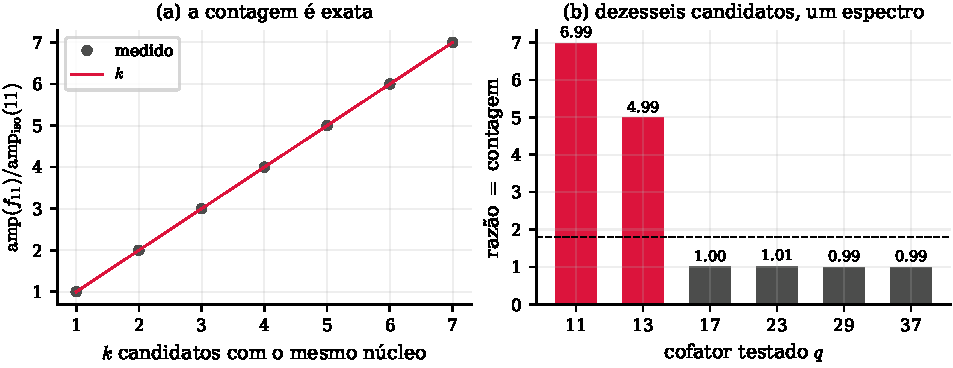
\includegraphics[width=0.95\textwidth]{figuras/f5_contagem.pdf}
\caption{(a) A razão medida em $\freq{11}$ para $k$ candidatos de núcleo comum,
com $k=1,\dots,7$; a reta é $\widehat k_{11}=k$. (b) Detecção em lote: dezesseis
candidatos, base $P=\{2,3,5,7\}$, um único espectro. As barras vermelhas são os
núcleos compartilhados, com altura igual à contagem.}
\label{fig:contagem}
\end{figure}

\begin{table}[htbp]
\centering
\small
\begin{tabular}{rrrr}
\toprule
núcleo $r$ & candidatos no lote & $\widehat k_r$ medido & erro \\
\midrule
$11$ & $7$ & $6{,}9897$ & $1{,}5\times10^{-3}$ \\
$13$ & $5$ & $4{,}9860$ & $2{,}8\times10^{-3}$ \\
$17$ & $1$ & $1{,}0010$ & $1{,}0\times10^{-3}$ \\
$23$ & $1$ & $1{,}0052$ & $5{,}2\times10^{-3}$ \\
$29$ & $1$ & $0{,}9932$ & $6{,}8\times10^{-3}$ \\
$37$ & $1$ & $0{,}9911$ & $8{,}9\times10^{-3}$ \\
\bottomrule
\end{tabular}
\caption{Leitura de um único espectro para dezesseis candidatos
($T=6500$, $\Delta t=5\times10^{-4}$). Os núcleos não compartilhados ficam em
torno de $1$, dentro do erro de lotação espectral.}
\label{tab:contagem}
\end{table}

\subsection{Três observações honestas}

\paragraph{A construção usa aritmética.} Para escrever \eqref{eq:colapsado} é
preciso calcular $v_p(m)$ de cada candidato, isto é, dividir. O que é espectral é a
\emph{medição}, não a preparação. A representação da Seção~\ref{sec:dicionario} é
fiel, mas não é gratuita: o núcleo é um dado aritmético antes de ser uma
frequência.

\paragraph{O que se mede é multiplicidade, não primalidade.} O detector conta
quantos candidatos compartilham um núcleo; ele não decide se o núcleo é primo nem
se os candidatos são. Se o núcleo for composto, o pico aparece em $\freq r$ com
$r$ composto, e a contagem continua correta. A proposição é sobre somas de termos
idênticos, não sobre aritmética dos termos.

\paragraph{O custo é o da janela.} Pela Proposição~\ref{prop:janela}, os núcleos
precisam estar resolvidos uns dos outros: se dois núcleos têm frequências muito
próximas, a faixa de leitura de um invade o outro e as contagens se contaminam. O
comprimento de janela necessário é $\tau$-como na Seção~\ref{sec:resolucao} — da
ordem do maior núcleo presente. Para lotes pequenos e núcleos pequenos, isso é
barato; para núcleos grandes, não é.

\subsection{Uma variante: potências}

A identidade não depende de os núcleos serem primos. Se um inteiro $m$ tem núcleo
$r=11^2$, o termo aparece em $\freq{121}$; se depois se remove um fator $11$, ele
migra para $\freq{11}$ e passa a somar com os demais. A contagem pode assim ser
feita em camadas: primeiro o núcleo completo, depois os núcleos sucessivos obtidos
removendo um fator de cada vez. Cada camada é um novo sinal
\eqref{eq:colapsado} e uma nova contagem exata.

Essa observação é o análogo, no dicionário, do que a fatoração por divisões
sucessivas faz na aritmética: ela desce a árvore de fatores por níveis. A
diferença é de leitura — na aritmética, o resultado é o quociente; aqui, é a
posição do pico no nível seguinte.

% ===========================================================================
\section{A assinatura de um par}\label{sec:assinatura}
% ===========================================================================

A última imagem é a de escala mais fina: não um bloco, mas um único par de
inteiros vizinhos. Ela mostra que a presença de um único tom é detectável, e a
que preço.

\subsection{O coeficiente em uma frequência}

Seja $N\ge2$ e considere o sinal dos primos até $N$,
\begin{equation}\label{eq:Rprimo}
  R(t) \;=\; -\sum_{\substack{p\le N\\ p\ \mathrm{primo}}}
  \frac{\cos\bigl(t\,\nfreq p\bigr)}{\sqrt p},
\end{equation}
que é a soma das componentes fundamentais \eqref{eq:serie}, com amplitude
$p^{-1/2}$, para os primos. Para $q\ge5$ defina
\[
  \hat a_q \;=\;
  \frac{\bigl|\hat R(\freq q)\bigr|}{T/(2\sqrt q)},
  \qquad
  \hat R(f) \;=\; \int_0^T R(t)\,e^{-2\pi i f t}\,dt ,
\]
isto é, a amplitude medida em $\freq q$ normalizada pela amplitude que um único
tom de tamanho $q$ produziria.

\begin{proposicao}\label{prop:gemeo}
Seja $q\ge5$ e defina
\[
  \varepsilon_q \;=\;
  \frac{2\sqrt q}{T}\sum_{\substack{p\le N\\ p\neq q}}
  \frac{1}{\sqrt p\,\bigl|\nfreq p-\nfreq q\bigr|}.
\]
Então
\[
  \bigl|\hat a_q - \mathbf 1_{q\in\mathcal P}\bigr| \;\le\; \varepsilon_q ,
\]
onde $\mathbf 1_{q\in\mathcal P}$ vale $1$ se $q$ é primo e $q\le N$, e $0$ caso
contrário. Além disso existem constantes absolutas $0<c<C$ com
\[
  \varepsilon_q \;\le\; C\,\frac{q\log q}{T},
  \qquad\text{e}\qquad
  \varepsilon_q \;\ge\; c\,\frac{q}{T}
  \ \text{ se } q-2 \text{ é primo}.
\]
\end{proposicao}

\begin{proof}
Escreva $\hat R=\sum_p \hat S_p$ com
$\hat S_p=-\frac{1}{2\sqrt p}\bigl[F(\nu_p-\nu_q)+F(-\nu_p-\nu_q)\bigr]$ e
$F(\alpha)=\bigl(e^{i\alpha T}-1\bigr)/(i\alpha)$, de modo que
$|F(\alpha)|\le 2/|\alpha|$ para $\alpha\neq0$ e $F(0)=T$.

\emph{Termo próprio.} Se $q\in\mathcal P$ então
$\hat S_q=-\tfrac{T}{2\sqrt q}\bigl(1+O((T\nu_q)^{-1})\bigr)$, e a normalização por
$T/(2\sqrt q)$ dá $1+O((T\nu_q)^{-1})$.

\emph{Termos alheios.} Para $p\neq q$,
\[
  \bigl|\hat S_p\bigr| \;\le\;
  \frac{1}{2\sqrt p}\Bigl(\frac{2}{|\nu_p-\nu_q|}+\frac{2}{\nu_p+\nu_q}\Bigr)
  \;\le\; \frac{1}{\sqrt p\,\bigl|\nfreq p-\nfreq q\bigr|}\,(1+\eta_p),
\]
com $\eta_p=O((T\nu_p)^{-1})$. Dividindo por $T/(2\sqrt q)$ obtém-se a soma que
define $\varepsilon_q$.

\emph{Cota superior.} Para $p$ com $|p-q|<q/2$, use
$|\nfreq p-\nfreq q|\ge |p-q|/\max(p,q)\ge |p-q|/(2q)$; então
\[
  \sum_{|p-q|<q/2}\frac{1}{\sqrt p\,\bigl|\nfreq p-\nfreq q\bigr|}
  \;\le\; \frac{2q}{\sqrt q}\sum_{p\neq q}\frac{1}{|p-q|}
  \;=\; O\bigl(\sqrt q\log q\bigr).
\]
Para $|p-q|\ge q/2$ tem-se $|\nfreq p-\nfreq q|\ge\log(3/2)$, e a soma restante é
$O\bigl(\sqrt q/\log q\bigr)$, já que $\sum_{p\le N}p^{-1/2}=O(\sqrt N/\log N)$ e
$N\asymp q$. Multiplicando por $2\sqrt q/T$ resulta $\varepsilon_q=O(q\log q/T)$.

\emph{Cota inferior.} Se $q-2$ é primo, o termo $p=q-2$ tem
$|\nfreq p-\nfreq q|=\log(1+2/(q-2))\le 2/(q-2)$, logo contribui com pelo menos
\[
  \frac{2\sqrt q}{T}\cdot\frac{1}{\sqrt q}\cdot\frac{q-2}{2}\;\ge\;\frac{q}{2T},
\]
independentemente de $T$.
\end{proof}

O conteúdo é o esperado do dicionário: a presença do tom é legível como uma
amplitude de ordem $1$; a ausência deixa apenas o vazamento dos tons vizinhos,
cuja amplitude relativa é da ordem de $q/T$. O parâmetro que governa a leitura é,
portanto, a razão $T/q$. A cota superior carrega um fator $\log q$ perdido na
estimativa grosseira da soma, mas a cota inferior mostra que a ordem correta é
$q/T$: o vizinho $q-2$ contribui sempre com essa ordem.

\subsection{O contraste}

A Proposição~\ref{prop:gemeo} dá o contraste entre os dois casos:
\[
  \frac{\text{sinal}}{\text{fundo}} \;\asymp\; \frac{1}{q/T} \;=\; \frac{T}{q}.
\]
Aumentar a janela aumenta o contraste linearmente, o que é o análogo, no nível
local, da lei de escala do Teorema~\ref{teo:custo}: para separar um tom do fundo
produzido pelos vizinhos, é preciso uma janela que cresça com o próprio $q$.

\subsection{Gêmeos e mistos}

A aplicação natural é a comparação de pares. Para cada primo $p\le N-2$, o par
$(p,p+2)$ é \emph{gêmeo} se $p+2$ é primo, e \emph{misto} caso contrário. A
Proposição~\ref{prop:gemeo} diz, sem mais hipóteses, que $\hat a_{p+2}\approx1$ no
primeiro caso e $\hat a_{p+2}\approx0$ no segundo, com folga da ordem de
$T/(p+2)$.

A Figura~\ref{fig:gemeos} mostra as duas distribuições para $N=300$ e
$T=6500$, medidas com o coeficiente exato (sem grade, isto é, avaliando a integral
\eqref{eq:Rprimo} diretamente na frequência). Os gêmeos se acumulam perto de $1$,
os mistos perto de $0$, e não há sobreposição.

\begin{figure}[htbp]
\centering
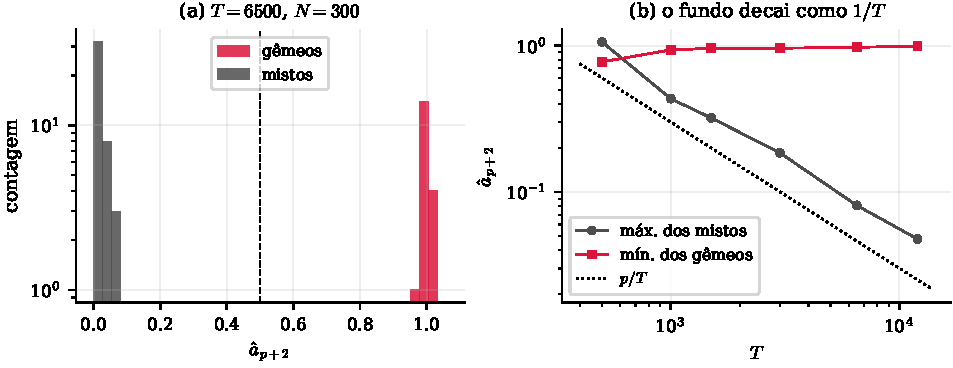
\includegraphics[width=0.95\textwidth]{figuras/f6_gemeos.pdf}
\caption{(a) Distribuição de $\hat a_{p+2}$ para os $62$ pares $(p,p+2)$ com
$p\le299$, com $T=6500$. (b) O máximo entre os mistos e o mínimo entre os gêmeos
em função de $T$; o fundo decai como $p/T$, como prevê a
Proposição~\ref{prop:gemeo}.}
\label{fig:gemeos}
\end{figure}

\begin{table}[htbp]
\centering
\small
\begin{tabular}{rrrr}
\toprule
$T$ & $\max$ dos mistos & $\min$ dos gêmeos & separação \\
\midrule
$500$   & $1{,}058$ & $0{,}774$ & falha \\
$1\,000$& $0{,}434$ & $0{,}934$ & completa \\
$1\,500$& $0{,}321$ & $0{,}958$ & completa \\
$3\,000$& $0{,}185$ & $0{,}959$ & completa \\
$6\,500$& $0{,}081$ & $0{,}973$ & completa \\
$12\,000$& $0{,}048$& $0{,}991$ & completa \\
\bottomrule
\end{tabular}
\caption{O fundo cai como $1/T$ e a separação se completa quando $T$ ultrapassa
algumas vezes $p_{\max}=299$.}
\label{tab:gemeos}
\end{table}

A assinatura é local: ela não usa a posição dos primos na reta, apenas a presença
ou ausência de um tom na frequência do par. É a instância mais fina do Teorema
\ref{teo:irred}: a irredutibilidade de $p+2$, traduzida em presença de frequência,
é legível para quem pode pagar a janela.

\subsection{Uma nota sobre a leitura}

Duas armadilhas práticas, ambas consequência da Proposição~\ref{prop:janela},
merecem registro porque afetam qualquer medição deste tipo.

A primeira é a grade. Se o coeficiente é avaliado em uma transformada discreta, a
frequência $\freq q$ raramente coincide com uma célula da grade, e o máximo lido
pode ser até $\operatorname{sinc}(\pi/2)\approx0{,}64$ do valor real. A correção é
avaliar o coeficiente na frequência exata, ou usar uma janela de afunilamento e
corrigir o ganho coerente.

A segunda é a faixa de leitura. Se a busca do pico varre $\pm W$ células e esse
intervalo inclui o pico do vizinho $q-2$, a leitura de um par misto herda a altura
do pico alheio — e a separação desaparece, como mostra a
Tabela~\ref{tab:janela}. Nenhum aumento de $T$ conserta isso: com $W$ fixo, a
condição $2W+1<T/(\pi q)$ é respeitada ou não.

Essas duas observações não são detalhes de implementação; são parte do conteúdo
matemático da representação, porque dizem em que condições a leitura de um
coeficiente corresponde ao termo que se quer medir.

% ===========================================================================
\section{Verificação e reprodutibilidade}\label{sec:verificacao}
% ===========================================================================

As figuras deste artigo são calculadas a partir das definições por um programa
curto em Python, e as tabelas por outro; ambos acompanham o texto. A aritmética da
Seção~\ref{sec:blocos} e as cotas da Seção~\ref{sec:geometria} foram também
verificadas de forma mecânica em Lean~4. Esta seção descreve o que foi calculado,
como, e o que a verificação formal cobre.

\subsection{Os programas}

\begin{sloppypar}
O material suplementar, disponível em
\url{https://github.com/tiagobandeira/analise-espectral-primos}, contém:
\end{sloppypar}

\begin{center}
\footnotesize
\begin{tabular}{llr}
\toprule
arquivo & o que calcula & tempo \\
\midrule
\texttt{figuras\_artigo.py} & as seis figuras (PDF vetorial) & $\approx 8$ min \\
\texttt{verificar\_teoremas.py} & as tabelas e as verificações V1--V5 & $\approx 2$ min \\
\bottomrule
\end{tabular}
\end{center}

O primeiro programa não depende de nenhuma biblioteca além de \texttt{numpy} e
\texttt{matplotlib}, e recalcula cada painel a partir da definição do sinal
\eqref{eq:Sm}: os logaritmos de módulo são somados termo a termo, as transformadas
são calculadas com \texttt{rfft} e as frequências convertidas por
$x=\operatorname{round}(e^{2\pi f})$. O segundo verifica por força bruta, para
blocos até $k=22$, que o menor fator primo de todo composto de $A_k$ está em
$\Seed_k$ (Lema~\ref{lema:bloco}), que o par de vizinhos inteiros de todo primo do
bloco é $\Seed_k$-suave (Lema~\ref{lema:qmaisum}) e que o mínimo de $\rB$ é
atingido em $q_k$ (Corolário~\ref{cor:min}).

\subsection{Os números das tabelas}

As Tabelas~\ref{tab:crivo}, \ref{tab:rho} e \ref{tab:lei} contêm os valores
medidos. A Tabela~\ref{tab:rho} é inteiramente explicada pelo
Teorema~\ref{teo:exato}: cada entrada é $g(q_k)$, calculada em precisão dupla, e a
coluna da cota é a expressão do Teorema~\ref{teo:cota}. A Tabela~\ref{tab:lei}
contém o par gargalo de cada semente, obtido por busca direta sobre os pares de
primos consecutivos.

A Tabela~\ref{tab:janela} e a Tabela~\ref{tab:gemeos} são medições, não
identidades: nelas há erro de leitura, e é justamente esse erro que a
Proposição~\ref{prop:janela} explica. Registramos nas duas tabelas o valor medido,
sem suavização.

\subsection{A verificação formal}

O núcleo da Seção~\ref{sec:geometria} e a aritmética da Seção~\ref{sec:blocos}
foram formalizados em Lean~4 sobre a biblioteca Mathlib \cite{mathlib}, sem
\texttt{sorry} e sem axiomas além dos da própria biblioteca. O Apêndice~\ref{ap:lean}
traz os enunciados exatos.

\begin{table}[htbp]
\centering
\small
\begin{tabular}{lll}
\toprule
resultado & declaração em Lean & status \\
\midrule
Lema~\ref{lema:bloco} (composto tem fator pequeno) &
\texttt{existe\_fator\_primo\_na\_semente} & provado \\
Teorema~\ref{teo:crivo} (crivo por blocos) &
\texttt{bloco\_primo\_iff} & provado \\
Teorema~\ref{teo:irred} (irredutibilidade) &
\texttt{logRedutivel\_iff} & provado \\
Lema~\ref{lema:vizinho} (vizinho inteiro) &
\texttt{log\_dist\_ge} & provado \\
Teorema~\ref{teo:cota} (cota uniforme) &
\texttt{cota\_rho} & provado \\
monotonia da cota em $k$ (auxiliar) &
\texttt{cota\_antitone} & provado \\
$\log(1+1/q)\ge 1/(q+1)$ &
\texttt{inv\_succ\_le\_log\_ratio} & provado \\
igualdade em $q+1$ &
\texttt{log\_dist\_succ\_eq} & provado \\
\bottomrule
\end{tabular}
\caption{O que a formalização cobre. As declarações residem em
\texttt{Espectral/Bloco.lean} e \texttt{Espectral/Rho.lean}, e compilam contra
\texttt{leanprover/lean4:v4.37.0-rc1} com Mathlib.}
\label{tab:lean}
\end{table}

O que a formalização \emph{não} cobre, e por quê:

\begin{itemize}[leftmargin=1.4em,itemsep=2pt]
\item A igualdade do Teorema~\ref{teo:exato} na forma completa exigiria definir
$\rB$ como mínimo sobre um conjunto de suaves; formalizamos as duas metades que a
demonstração usa — a cota inferior para todo inteiro (Lema~\ref{lema:vizinho}) e o
fato de a cota ser atingida em $q+1$ —, que é o conteúdo matemático. O passo
final, ``logo o mínimo é esse valor'', é imediato no papel.
\item A suavidade de $q+1$ (Lema~\ref{lema:qmaisum}) é aritmética elementar mas
exige a maquinaria de fatoração de Mathlib; deixamo-la no papel.
\item As Proposições~\ref{prop:gemeo} e \ref{prop:janela} são afirmações sobre
integrais de somas finitas de cossenos. Formalizá-las exigiria a teoria de
integrais de Riemann para funções oscilatórias, com custo desproporcional ao
conteúdo, que é uma desigualdade triangular e $|F(\alpha)|\le2/|\alpha|$.
\end{itemize}

\subsection{Como reproduzir}

\begin{center}
\begin{minipage}{0.95\textwidth}
\footnotesize
\begin{verbatim}
# figuras (Python 3.11+, numpy, matplotlib)
python artigo/experimentos/figuras_artigo.py

# tabelas e verificações por força bruta
python artigo/experimentos/verificar_teoremas.py

# formalização (Lean 4 + Mathlib)
cd formalizacao && lake exe cache get && lake build
\end{verbatim}
\end{minipage}
\end{center}

Nenhum dos cálculos usa amostragem aleatória: todos são determinísticos, e os
valores das tabelas são reprodutíveis bit a bit em precisão dupla. Os arquivos
\texttt{.json} produzidos pelos programas contêm os valores brutos de cada medida
citada no texto.

% ===========================================================================
\section{O que a representação sugere}\label{sec:perspectiva}
% ===========================================================================

\subsection{O dicionário em resumo}

O artigo construiu uma tradução e mediu suas consequências. A tabela abaixo
resume o que foi traduzido.

\begin{center}
\small
\begin{tabular}{ll}
\toprule
aritmética & reta (frequência) \\
\midrule
inteiro $m$ & ponto $\nfreq m=\log m$ \\
produto $mn$ & soma $\nfreq m+\nfreq n$ \\
$B$-suavidade & pertencer ao reticulado $\Lat(B)$ \\
ser composto & ser soma de geradores \\
ser primo & ser irredutível \\
divisibilidade por $p$ & pertencer a $\Lat(\{p\})$ \\
semente $\Seed_k$ & reticulado do bloco anterior \\
margem de classificação & $\rB_{\min}(k)=g(q_k)$ \\
\bottomrule
\end{tabular}
\end{center}

Nenhuma linha dessa tabela é profunda isoladamente: todas são o Teorema
Fundamental da Aritmética visto por logaritmos. O que a tabela oferece é uma
\emph{linguagem}, e a linguagem tem consequências que a notação multiplicativa não
tem: ela permite falar de distância, de resolução, de superposição e de contagem.
Os Teoremas~\ref{teo:exato} e \ref{teo:custo} e as
Proposições~\ref{prop:ganho} e \ref{prop:gemeo} são exemplos dessas consequências.

\subsection{Perguntas que ficam}

\paragraph{Outras bases.} A partição binária não é a única possível. Para uma base
$b\ge2$, o bloco $[b^k,b^{k+1})$ tem comprimento $b^k(b-1)$, e o menor fator de um
composto é $<b^{(k+1)/2}$; a semente correspondente é $\{p<b^k\}$. O análogo do
Teorema~\ref{teo:cota} vale com $b$ no lugar de $2$, mas a geometria muda: a
margem passa a depender de $b$, e não sabemos se o análogo do
Teorema~\ref{teo:exato} vale para $b>2$ — o vizinho $q+1$ deixa de estar sempre no
reticulado quando $q$ não é ímpar.

\paragraph{Outros crivos.} O crivo de Eratóstenes é o que a partição binária
organiza. O que acontece com crivos de roda (\emph{wheel sieves}), que riscam
múltiplos de vários primos de uma vez? A imagem correspondente seria uma soma de
tons em frequências de produtos, e a contagem coerente sugere que a altura dos
picos mediria quantos candidatos caem em cada classe residual.

\paragraph{Órbitas e a função de Dickman.} A contagem $k_r$ da
Proposição~\ref{prop:ganho} é o tamanho de uma órbita $\mathcal O_r$. Para $P$ fixo
e $m\le X$, essa contagem é o número de inteiros de $\mathcal O_r$ abaixo de $X$,
que é exatamente o objeto da teoria de números suaves e da função de
Dickman--de Bruijn $\Psi(X,y)$ \cite{tenenbaum}. A representação espectral dá a
$\Psi$ uma leitura: a altura do pico em $\freq r$ é $\Psi$-local.

\paragraph{A assinatura de pares gêmeos.} A Proposição~\ref{prop:gemeo} dá a lei
$q/T$ para o fundo. A constante ótima — a que aparece na
Tabela~\ref{tab:gemeos} como fator entre $q/T$ e o máximo medido, da ordem de
$1{,}8$ — não foi determinada. Determiná-la exigiria controlar a interferência
conjunta de todos os primos do sinal, e não só do vizinho imediato.

\paragraph{Aplicações visuais.} As figuras deste artigo foram feitas para serem
olhadas, mas cada uma delas é o resultado de um cálculo simples e curto. Um
instrumento interativo — em que o leitor escolhe $p$, o número de primos, a janela
e a faixa de leitura — permitiria percorrer a transição entre ``os pares se
fundem'' e ``os pares se separam'' que a Figura~\ref{fig:resolucao} mostra em dois
instantâneos. A Proposição~\ref{prop:janela} dá o critério exato para colorir essa
transição.

\subsection{O que este artigo não é}

Vale ser explícito sobre o alcance do que foi feito, para que o leitor saiba o que
esperar daqui.

A representação é fiel: os primos de um bloco aparecem como picos isolados, e
cada afirmação estrutural sobre eles tem uma tradução geométrica exata. Mas ela
não é um algoritmo competitivo. A aritmética decide em $O(\sqrt m)$ o que a
imagem exige uma janela de tamanho $\Theta(m)$ para mostrar
(Corolário~\ref{cor:local}). O valor do dicionário está em outro lugar: em tornar
visíveis relações que a notação multiplicativa esconde, e em dar a cada uma delas
uma lei quantitativa.

É, nesse sentido, o tipo de matemática que se faz para entender uma estrutura, e
não para calcular com ela. A estrutura em questão — a irredutibilidade dos
inteiros — é bem conhecida; o que é novo aqui é o ângulo, e o que o ângulo revela
são grandezas que não apareciam antes: a margem $g(q_k)$, o comprimento
$\tau(\Seed_k)$, o contraste $T/q$. Essas grandezas são as mesmas que governam
qualquer tentativa de ler aritmética por frequência, e é por isso que vale
registrá-las.


\appendix
% ===========================================================================
\section{Os enunciados verificados}\label{ap:lean}
% ===========================================================================

Reproduzimos aqui os enunciados das declarações verificadas em Lean~4, em notação
matemática. O código-fonte completo, com as demonstrações, está em
\path{formalizacao/Espectral/Bloco.lean} e
\path{formalizacao/Espectral/Rho.lean}, no material suplementar; os nomes das
declarações são os que aparecem nos títulos abaixo.

\subsection*{Lema do bloco (\texttt{existe\_fator\_primo\_na\_semente})}

\noindent Para todo $k\ge1$ e todo $m$ inteiro,
\[
  2^k \le m < 2^{k+1} \ \wedge\ \lnot\,\mathrm{Primo}(m)
  \;\Longrightarrow\;
  \exists p,\ \mathrm{Primo}(p)\ \wedge\ p\mid m\ \wedge\ p<2^k .
\]

\subsection*{Crivo por blocos (\texttt{bloco\_primo\_iff})}

\noindent Para todo $k\ge1$ e todo $m$ com $2^k\le m<2^{k+1}$,
\[
  \mathrm{Primo}(m)
  \;\Longleftrightarrow\;
  \forall p,\ \mathrm{Primo}(p)\ \wedge\ p\mid m \ \Rightarrow\ 2^k\le p .
\]

\subsection*{Irredutibilidade logarítmica (\texttt{logRedutivel\_iff})}

\noindent Um inteiro $m$ é \emph{logaritmicamente redutível} se existem um
conjunto finito $s$ de primos, expoentes $e\colon s\to\N_{>0}$ e a identidade
$\log m=\sum_{p\in s}e(p)\log p$ com $p<m$ para todo $p\in s$. O enunciado
verificado é: para todo $m\ge2$,
\[
  \mathrm{LogRedutivel}(m)
  \;\Longleftrightarrow\;
  \lnot\,\mathrm{Primo}(m).
\]

\subsection*{Vizinho inteiro (\texttt{log\_dist\_ge}, \texttt{log\_dist\_succ\_eq})}

\noindent Para inteiros $q,m\ge2$ com $m\neq q$,
\[
  \log(q+1)-\log q \;\le\; \bigl|\log q-\log m\bigr| ,
\]
e a igualdade vale para $m=q+1$:
\[
  \bigl|\log q-\log(q+1)\bigr| \;=\; \log(q+1)-\log q .
\]

\subsection*{Desigualdade auxiliar (\texttt{inv\_succ\_le\_log\_ratio})}

\noindent Para todo inteiro $q\ge1$,
\[
  \frac{1}{q+1} \;\le\; \log(q+1)-\log q .
\]

\subsection*{Cota uniforme (\texttt{cota\_rho})}

\noindent Para $k\ge1$, $q$ primo com $2^k\le q<2^{k+1}$ e $m\ge2$ com $m\neq q$,
\[
  \frac{1}{2^{k+1}(k+1)\log 2}
  \;\le\;
  \frac{\bigl|\log q-\log m\bigr|}{\log q} .
\]
Como $\rB(q)$ é o mínimo dessa quantidade sobre os inteiros do reticulado, a
desigualdade implica a cota do Teorema~\ref{teo:cota}.

\subsection*{Monotonia da cota (\texttt{cota\_antitone})}

\noindent Para $1\le k\le k'$,
\[
  \frac{1}{2^{k'+1}(k'+1)\log 2}
  \;\le\;
  \frac{1}{2^{k+1}(k+1)\log 2} .
\]
Ou seja: a cota do Teorema~\ref{teo:cota} — e com ela a margem que separa primos
de compostos — decresce com o tamanho do bloco, como o
Corolário~\ref{cor:assint} quantifica.

\subsection*{O que não está coberto}

A igualdade do Teorema~\ref{teo:exato} na forma completa exigiria definir $\rB$
como mínimo sobre um conjunto de números suaves, o que exige decidir suavidade em
tempo de prova. Formalizamos as duas metades que a demonstração usa — a cota
inferior para todo inteiro e o fato de a cota ser atingida em $q+1$ —, que é o
conteúdo matemático; o passo final, ``logo o mínimo é esse valor'', é imediato no
papel e verificado numericamente na Tabela~\ref{tab:dadosrho}. O
Lema~\ref{lema:qmaisum} (suavidade de $q+1$) também ficou no papel: é aritmética
elementar, mas exige a maquinaria de fatoração da biblioteca.

\subsection*{Como compilar}

\begin{center}
\begin{minipage}{0.9\textwidth}
\begin{verbatim}
cd formalizacao
lake exe cache get     # oleans pré-compilados do Mathlib (~1 GB)
lake build
\end{verbatim}
\end{minipage}
\end{center}

\noindent A formalização usa \texttt{leanprover/lean4:v4.37.0-rc1} com Mathlib. As
três compilações terminam sem erros e sem avisos; não há \texttt{sorry}.

% ===========================================================================
\section{Dados numéricos}\label{ap:dados}
% ===========================================================================

As duas tabelas abaixo contêm os valores completos usados nas
Figuras~\ref{fig:reticulado} e \ref{fig:lei}. Ambos são calculados diretamente
pelas fórmulas dos Teoremas~\ref{teo:exato} e \ref{teo:custo}: a primeira coluna de
cada uma é uma contagem de primos, as demais são avaliações de funções
elementares.

\begin{table}[htbp]
\centering
\small
\begin{tabular}{rrrrr}
\toprule
$k$ & $q_k=\max\Pi_k$ & $\rB_{\min}(k)=g(q_k)$ & cota & razão \\
\midrule
$2$  & $7$        & $6{,}862\times10^{-2}$ & $6{,}011\times10^{-2}$ & 1,142 \\
$3$  & $13$       & $2{,}889\times10^{-2}$ & $2{,}254\times10^{-2}$ & 1,282 \\
$4$  & $31$       & $9{,}245\times10^{-3}$ & $9{,}017\times10^{-3}$ & 1,025 \\
$5$  & $61$       & $3{,}956\times10^{-3}$ & $3{,}757\times10^{-3}$ & 1,053 \\
$6$  & $127$      & $1{,}619\times10^{-3}$ & $1{,}610\times10^{-3}$ & 1,006 \\
$7$  & $251$      & $7{,}196\times10^{-4}$ & $7{,}044\times10^{-4}$ & 1,022 \\
$8$  & $509$      & $3{,}149\times10^{-4}$ & $3{,}131\times10^{-4}$ & 1,006 \\
$9$  & $1\,021$   & $1{,}413\times10^{-4}$ & $1{,}409\times10^{-4}$ & 1,003 \\
$10$ & $2\,039$   & $6{,}434\times10^{-5}$ & $6{,}404\times10^{-5}$ & 1,005 \\
$11$ & $4\,093$   & $2{,}937\times10^{-5}$ & $2{,}935\times10^{-5}$ & 1,001 \\
$12$ & $8\,191$   & $1{,}355\times10^{-5}$ & $1{,}355\times10^{-5}$ & 1,000 \\
$13$ & $16\,381$  & $6{,}291\times10^{-6}$ & $6{,}290\times10^{-6}$ & 1,000 \\
$14$ & $32\,749$  & $2{,}937\times10^{-6}$ & $2{,}935\times10^{-6}$ & 1,001 \\
$15$ & $65\,521$  & $1{,}376\times10^{-6}$ & $1{,}376\times10^{-6}$ & 1,000 \\
$16$ & $131\,071$ & $6{,}475\times10^{-7}$ & $6{,}475\times10^{-7}$ & 1,000 \\
$17$ & $262\,139$ & $3{,}058\times10^{-7}$ & $3{,}058\times10^{-7}$ & 1,000 \\
$18$ & $524\,287$ & $1{,}448\times10^{-7}$ & $1{,}448\times10^{-7}$ & 1,000 \\
\bottomrule
\end{tabular}
\caption{$\rB_{\min}(k)$, a cota do Teorema~\ref{teo:cota} e a razão entre as
duas. Note que em $k=16$ o valor cruza $10^{-6}$.}
\label{tab:dadosrho}
\end{table}

\begin{table}[htbp]
\centering
\small
\begin{tabular}{rrrrr}
\toprule
$n$ & par gargalo de $\Seed_n$ & $\tau(\Seed_n)$ & $\pi\,q_{\text{gêmeo}}$ & razão \\
\midrule
$4$  & $(5,7)$               & $18{,}7$      & $22{,}0$      & 0,851 \\
$5$  & $(11,13)$             & $37{,}6$      & $40{,}8$      & 0,920 \\
$6$  & $(29,31)$             & $94{,}2$      & $97{,}4$      & 0,967 \\
$7$  & $(59,61)$             & $188{,}5$     & $191{,}6$     & 0,984 \\
$8$  & $(107,109)$           & $339{,}3$     & $342{,}4$     & 0,991 \\
$9$  & $(239,241)$           & $754{,}0$     & $757{,}1$     & 0,996 \\
$10$ & $(461,463)$           & $1\,451{,}4$  & $1\,454{,}6$  & 0,998 \\
$11$ & $(1\,019,1\,021)$     & $3\,204{,}4$  & $3\,207{,}6$  & 0,999 \\
$12$ & $(2\,027,2\,029)$     & $6\,371{,}1$  & $6\,374{,}3$  & 1,000 \\
$13$ & $(4\,091,4\,093)$     & $12\,855{,}4$ & $12\,858{,}5$ & 1,000 \\
$14$ & $(8\,087,8\,089)$     & $25\,409{,}2$ & $25\,412{,}3$ & 1,000 \\
\bottomrule
\end{tabular}
\caption{A janela exigida por $\Seed_n$ e sua relação com $\pi q_{\text{gêmeo}}$,
onde $q_{\text{gêmeo}}$ é o maior elemento de um par de gêmeos da semente.}
\label{tab:dadoslei}
\end{table}

As duas tabelas foram verificadas por programa independente, que recalcula cada
entrada a partir das definições (Seção~\ref{sec:verificacao}). Os valores de
$\tau$ são obtidos por busca direta sobre os pares de primos consecutivos de cada
semente, sem usar a forma assintótica.


\begin{thebibliography}{99}

\bibitem{baker} A.~Baker, \emph{Transcendental Number Theory},
Cambridge University Press, 1975.

\bibitem{hildebrand} A.~J.~Hildebrand, G.~E.~Andrews, \emph{Number Theory},
Dover, 1994.

\bibitem{lang} S.~Lang, \emph{Algebraic Number Theory}, 2.~ed.,
Springer, 1994.

\bibitem{montgomery} H.~L.~Montgomery, R.~C.~Vaughan,
\emph{Multiplicative Number Theory I: Classical Theory},
Cambridge University Press, 2007.

\bibitem{tenenbaum} G.~Tenenbaum, \emph{Introduction to Analytic and
Probabilistic Number Theory}, 3.~ed., American Mathematical Society, 2015.

\bibitem{titchmarsh} E.~C.~Titchmarsh, \emph{The Theory of the Riemann
Zeta-Function}, 2.~ed., Oxford University Press, 1986.

\bibitem{korner} T.~W.~K\"orner, \emph{Fourier Analysis}, Cambridge
University Press, 1988.

\bibitem{mathlib} The Mathlib Community, \emph{The Lean Mathematical Library},
in: Proceedings of CPP 2020, ACM, 2020.

\end{thebibliography}

\end{document}
